\documentclass[a4paper,12pt]{article}
\usepackage{../packages/coursCollege}
\newcommand{\Chapitre}{Limites et continuité}
\renewcommand{\path}{../}

\usepackage[    %backend=biber, 
    natbib=true,
    style=numeric,
    sorting=none]{biblatex}  % Load biblatex for bibliography handling
\addbibresource{biblio-der.bib}  
\renewcommand\refname{Sources}
\renewcommand{\cours}{3MA1~--~EG~--~ns~--~2025-2026}
\begin{document}
\tocloftpagestyle{fancy}
% Reduce space between section entries
\setlength{\cftbeforesecskip}{2pt}

% Reduce indentation for section entries
\setlength{\cftsecindent}{1em}

\begin{center}
	{\bfseries \Huge Chapitre 1~: \\Fonctions continues et calcul de limites}
	

	\vspace{1cm}
\begin{tikzpicture}[scale=4]
  % unit circle, solid

  \node[inner sep=0] at (0,0) {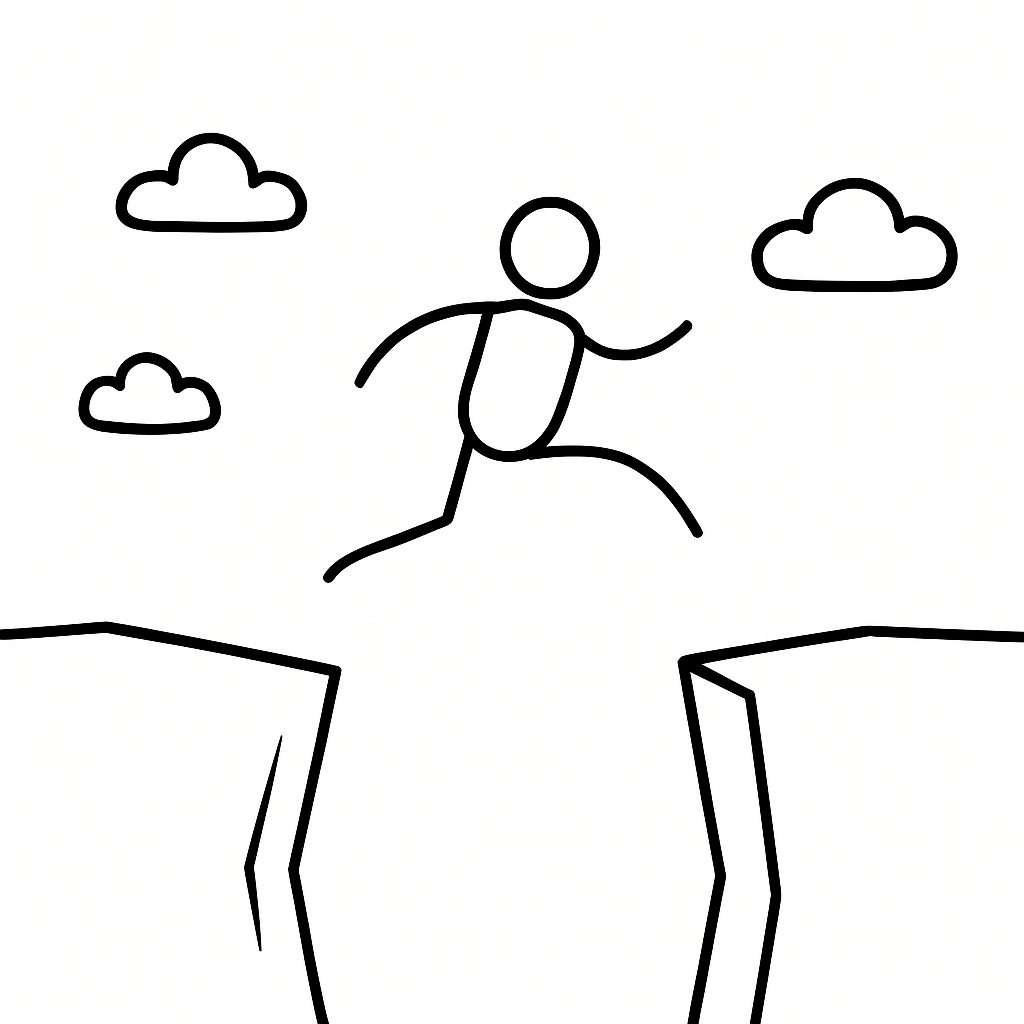
\includegraphics[width=9cm]{../medias/3M/limites/intro}};
  \draw[very thick] (0,0) circle (1);

  % inscribed n-gons, dashed
  \foreach \n in {4,5,6,7,8,9,10,20,30,40} {
    \draw[thick, dashed]
      (0:1)
      \foreach \i in {1,...,\numexpr\n-1\relax}
        { -- ({\i*360/\n}:1) }
      -- cycle;
  }
\end{tikzpicture}
\end{center}
\vspace{-1cm}
\tableofcontents

{\footnotesize Version du \today}
\newpage
\section*{Prérequis}
Avant de commencer ce chapitre, je m'assure d'être capable de 
\bigskip


\begin{tblr}{
  colspec = {|l|X[2]|c|c|},     % Adjusted column widths
  row{1} = {bg=gray!20, font=\bfseries}, % Header styling
  rows = {valign=m, ht=2cm},    % Minimum row height for QR codes
  vlines,
  hlines,
  width = \textwidth,           % Table spans full text width
}
%------------ Header -------------------------------------------------
Catégorie & 
Compétence & 
QR Code & 
Validation \\
%------------ Calcul numérique ---------------------------------------
\SetCell[r=2]{l, bg=blue!10} {\textbf{Calcul\\numérique}} &
Calculer avec des fractions &
\qrcode[height=2.5cm]{https://coopmaths.fr/alea/?uuid=374b6&id=10NO5-4&n=10&d=10&s=7&cd=1&uuid=72ce7&id=10NO5-6&n=4&d=10&s=3&s2=true&s3=true&s4=3&cd=1&lang=fr-CH&v=eleve&es=2211001&title=} &
\checkBox \\
&
Calculer avec des racines et les conjugués &
\qrcode[height=2.5cm]{https://coopmaths.fr/alea/?uuid=d9495&id=11NO1-6&uuid=99b29&id=11NO1-5&n=8&d=10&s=1&cd=1&uuid=4771d&id=1mCN-12&n=3&d=10&s=4&cd=1&lang=fr-CH&v=eleve&es=2211001&title=} &
\checkBox \\
%------------ Algèbre ------------------------------------------------
\SetCell[r=2]{l, bg=green!10} {\textbf{Algèbre}} &
Factoriser un polynôme en déterminant ses racines &
\qrcode[height=2.5cm]{https://coopmaths.fr/alea/?uuid=a8e1b&id=11FA10-13&lang=fr-CH&v=eleve&es=2211001&title=} &
\checkBox \\
&
Effectuer la division polynomiale &
\qrcode[height=2.5cm]{https://coopmaths.fr/alea/?uuid=ad6a2&id=HPC100&n=3&d=10&s=1&cd=1&v=eleve&es=2211001&title=} &
\checkBox \\
%------------ Fonctions ----------------------------------------------
\SetCell[r=2]{l, bg=orange!10} {\textbf{Fonctions}} &
Déterminer le domaine de définition d'une fonction &
\qrcode[height=2.5cm]{https://coopmaths.fr/alea/?uuid=6ea62&id=1mF1-12&n=12&d=10&s=8&s2=3&cd=1&lang=fr-CH&v=eleve&es=2211001&title=} &
\checkBox \\
&
« Étudier » une fonction du second degré &
\qrcode[height=2.5cm]{https://coopmaths.fr/alea/?uuid=5ea23&id=1mF3-3&lang=fr-CH&v=eleve&es=2211001&title=} &
\checkBox
\end{tblr}

\vspace{1em}

\textit{Note: Scannez les codes QR pour accéder aux ressources d'apprentissage correspondantes.}

\newpage
\section{Continuité}
\subsection{Définition intuitive et exemples}
\label{sec:continuite}
\begin{definition}
	\tcblower
	Un \emph{voisinage} d'un nombre réel $a$ est un intervalle ouvert qui contient $a$.
\end{definition}
\begin{exemple}
	\tcblower
		Les intervalles ouverts $]1\,{;}\,4[$ et $]2{,}9999\,{;}\,3{,}000000001[$ sont des voisinages de $3$.
\end{exemple}
\begin{remarque}
	\tcblower
 Par définition, un voisinage d'un nombre réel $a$ contient une infinité de nombres plus petit et plus grand que $a$. 
\end{remarque}
\begin{definition}
	\tcblower
	On dit qu'une fonction est \emph{définie au voisinage} d'un nombre réel $a$ ssi il existe un voisinage de $a$ sur lequel la fonction est définie, sauf peut-être en~$a$.
\end{definition}

\begin{definition}
\tcblower
Soit $f : I \to \mathbb{R}$ une fonction réelle (donc $I \subset \mathbb{R}$) et $a \in I$.  
On dit que $f$ est continue en $a$ ssi il existe un voisinage de $a$ tel que « une représentation graphique de $f$ dans ce voisinage peut être dessinée sans lever le crayon ».  
\end{definition}
\begin{remarque}
	\tcblower
	Cette définition n'est pas formelle. Un des objectifs de ce chapitre est d'étudier l'outil « limite » qui permet de caractériser la continuité.
	\end{remarque}

\begin{definition}
	\tcblower
	\
	$f$ est continue sur $I$ un intervalle $I\subset \mathbb{R}$ ssi $f$ est continue en tout point de~$I$.
\end{definition}



\begin{exemple}[label=ex:continuiteintro]
	\tcblower
	\begin{tasks}(2)
	\task 

	\begin{tikzpicture}[>=stealth]
% ------------------------------------------------------------------
% 1 ── no value at a (open circle)
\begin{axis}[
    name=G1,
    width=5.5cm,height=5.5cm,
    axis lines=middle, axis line style={->},
    xmin=-1,xmax=4, ymin=-1,ymax=2,
    xtick=\empty, ytick=\empty,
    clip=false]
  \addplot[smooth,thick] coordinates
      {(-1,-1) (0,-0.2) (1,0.5) (2,1.2) (3,1.4) (4,1.2)};
  \draw[dashed] (axis cs:2,0) -- (axis cs:2,1.2);
  \draw[dashed] (axis cs:0,1.2) -- (axis cs:2,1.2);
  \draw[fill=white,thick] (axis cs:2,1.2) circle (2pt); % ∘
  \node[below] at (axis cs:2,0) {$a$};
  \node[left]  at (axis cs:0,1.2) {$b$};
\end{axis}
\end{tikzpicture}

$f$ n'est pas continue en $a$, car $f$ n'est pas définie en $a$.
\task 




\begin{tikzpicture}[>=stealth]

	% ------------------------------------------------------------------
% 2 ── continuous, piecewise-linear peak
\begin{axis}[
    at={(G1.east)}, xshift=1.5cm,
    width=5.5cm,height=5.5cm,
    axis lines=middle, axis line style={->},
    xmin=-1,xmax=5, ymin=-1,ymax=2,
    xtick=\empty, ytick=\empty,
    clip=false]
  \addplot[thick] coordinates {(-1,-0.3) (2,1.4) (5,-0.6)};
  \draw[dashed] (axis cs:2,0) -- (axis cs:2,1.4);
  \draw[dashed] (axis cs:-0.1,1.4) -- (axis cs:2,1.4);
  \draw[fill=black] (axis cs:2,1.4) circle (2pt);
  \node[below] at (axis cs:2,0) {$a$};
  \node[left]  at (axis cs:0,1.4) {$b$};
\end{axis}
\end{tikzpicture}

$f$ est continue en $a$.

\task 

\begin{tikzpicture}[>=stealth]
	\begin{axis}[
    at={(G1 -| G1.east)}, xshift=3cm,
    width=5.5cm,height=5.5cm,
    axis lines=middle, axis line style={->},
    xmin=-1,xmax=4, ymin=-1,ymax=2,
    xtick=\empty, ytick=\empty,
    clip=false]
  \addplot[smooth,thick,domain=-1:2,samples=80] {0.6+0.5*x-0.2*x^2};
  \addplot[smooth,thick,domain=2:4,samples=80] {0.06*(x-2)^2+0.15*(x-2)+0};
  % points & guides
  \draw[dashed] (axis cs:2,0) -- (axis cs:2,0.8);
  \draw[dashed] (axis cs:0,0.8) -- (axis cs:2,0.8);
  \draw[dashed] (axis cs:0,0) -- (axis cs:2,0);
  \draw[fill=white,thick] (axis cs:2,0) circle (2pt);   % open
  \draw[fill=black]       (axis cs:2,0.8) circle (2pt); % closed
  \node[below] at (axis cs:2,0) {$a$};
  \node[left]  at (axis cs:0,0.8) {$b$};
\end{axis}
\end{tikzpicture}

$f$ n'est pas continue en $a$.

\task 

\begin{tikzpicture}[>=stealth]
	\begin{axis}[
    at={(G1.south)}, yshift=-1.5cm,
    width=5.5cm,height=5.5cm,
    axis lines=middle, axis line style={->},
    xmin=-1,xmax=4, ymin=-1,ymax=2,
    xtick=\empty, ytick=\empty,
    clip=false]
  \addplot[smooth,thick,domain=-1:4,samples=100]
      {-0.25*(x-2)^2+1.2};
  \draw[dashed] (axis cs:2,0) -- (axis cs:2,1.2);
  \draw[dashed] (axis cs:0,1.2) -- (axis cs:2,1.2);
  \draw[dashed] (axis cs:0,0.5) -- (axis cs:2,0.5);
  \draw[dashed] (axis cs:0,0.0) -- (axis cs:2,0.0);
  \draw[fill=white,thick] (axis cs:2,1.2) circle (2pt); % open
  \draw[fill=black]       (axis cs:2,0.5) circle (2pt); % value
  \node[below] at (axis cs:2,0) {$a$};
  \node[left]  at (axis cs:0,1.2) {$b$};
  \node[left]  at (axis cs:0,0.5) {$c$};
\end{axis}
\end{tikzpicture}

$f$ n'est pas continue en $a$.

\end{tasks}
\end{exemple}
\begin{exemplesuite}
	\tcblower
	\begin{tasks}(2)

		\task[e)] 

\begin{tikzpicture}[>=stealth]
	\begin{axis}[
    at={(G1 -| G1.east |- G1.south)}, xshift=3cm,
    width=5.5cm,height=5.5cm,
    axis lines=middle, axis line style={->},
    xmin=-1,xmax=4, ymin=-1,ymax=2,
    xtick=\empty, ytick=\empty,
    clip=false]
  \addplot[smooth,thick,domain=-1:4,samples=100] {0.1*(x-2)^3 -0.5*(x-2) +0.3};
  \draw[dashed] (axis cs:2,0.3) -- (axis cs:0,0.3);
  \draw[dashed] (axis cs:2,0) -- (axis cs:2,0.3);
  \draw[fill=black] (axis cs:2,0.3) circle (2pt);
  \node[below] at (axis cs:2,0) {$a$};
  \node[above left]  at (axis cs:0,0.3) {$b$};
\end{axis}
\end{tikzpicture}

$f$ est continue en $a$.

\task[f)] 

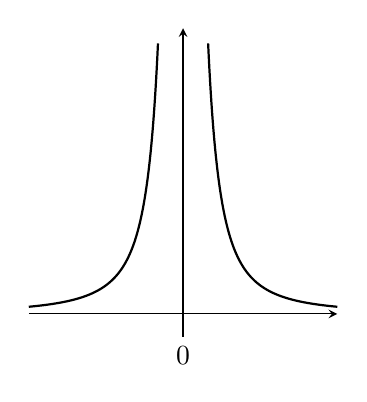
\begin{tikzpicture}[>=stealth]
\begin{axis}[
    width=5.5cm,height=5.5cm,
    axis lines=middle, axis line style={->},
    xmin=-4,xmax=4, ymin=-0.2,ymax=2.5,
    xtick=\empty, ytick=\empty,
    clip=false]
  % 1/x² left branch
  \addplot[domain=-4:-0.65,samples=200,thick] {1/(x^2)};
  % 1/x² right branch
  \addplot[domain=0.65:4,samples=200,thick] {1/(x^2)};
  % vertical asymptote x = 0
  \draw[dashed] (axis cs:0,-0.2) -- (axis cs:0,2.5);
  \node[below] at (axis cs:0,-0.2) {$0$};
\end{axis}
\end{tikzpicture}

$f$ n'est pas continue en $0$, car $f$ n'est pas définie en $0$.

	\end{tasks}
\end{exemplesuite}


\subsection{Théorème de la valeur intermédiaire}
\begin{thm}
Théorème de la valeur intermédiaire
\tcblower
Si $f : I \to \mathbb{R}$ est une fonction continue sur $\interval{a}{b}$, alors la fonction $f$
\begin{itemize}
	\item est bornée sur $\interval{a}{b}$
	\item possède un minimum $m$ et un maximum $M$ sur $\interval{a}{b}$
	\item prend au moins une fois toutes les valeurs comprises entre $m$ et $M$.
\end{itemize}
En d'autres termes, $f(\interval{a}{b}) = \interval{m}{M}$
\end{thm}
\begin{exemple}
	\tcblower
	Soit $f:\interval{0}{1}\rightarrow\interval{0}{1}$ une fonction continue. Montrer qu'il existe $a\in\interval{0}{1}$ tel que $f(a)=a$.
	\vspace{6cm}
\end{exemple}
\begin{coro}
	\tcblower
	Soit $f$ une fonction continue sur un intervalle $\interval{a}{b}$ si 
	\[f(a)\geq 0 \text{ et } f(b) \leq 0 \text{ {\bfseries ou} } f(a)\leq 0 \text{ et } f(b)\geq 0,\]
	alors $f$ s'annule sur $\interval{a}{b}$, c'est-à-dire qu'il existe $c\in \interval{a}{b}$ tel que $f(c)=0$. 
\end{coro}
\begin{remarque}
	\tcblower
Si l'hypothèse de continuité n'est pas vérifiée, ces deux résultats ne sont plus vrais~!
\end{remarque}



\section{Limites en un nombre}
\subsection{Un exemple introductif}
\begin{exemple}
	\tcblower

	{\bfseries Exemple introductif} -- 
	Considérons la fonction définie par

	\begin{align*}
		f : \mathbb{R}_+ \setminus \{1; 4\} &\to \mathbb{R}\\
		x &\mapsto \dfrac{3(1-x)}{(\sqrt{x}-1)(x-4)}
	\end{align*}

Nous allons étudier le comportement de cette fonction aux bords de son ensemble de définition, c'est-à-dire en 
\begin{itemize}
\item en $x = 1$ puis $x = 4$ (valeurs interdites)
\item en $x=0$ et finalement en $x \to +\infty$
\end{itemize}

\begin{tasks}(1)
\task Si on évalue la fonction $f$ pour les deux premières valeurs, on risque d'obtenir des réponses peu concluantes :

\[f(1) =\ligne{1} f(4) = \ligne{1}\]

\task Utilisons des tableaux de valeurs :
\begin{itemize}

\item S'approcher de la valeur 1 en venant depuis la gauche $(x \to 1^-)$ et depuis la droite $(x \to 1^+)$

\begin{center}
\begin{tabular}{|c|c|c|c|c|c|}
\hline
& \multicolumn{2}{c|}{gauche $\to$} & & \multicolumn{2}{c|}{$\leftarrow$ droite} \\
\hline
$x$ & $0,9$ & $0,99$ & $1$ & $1,01$ & $1,1$ \\
\hline
$f(x)$ & $1,886$ & $1,989$ & ??? & $2,012$ & $2,12$ \\
\hline
\end{tabular}
\end{center}

Ainsi, il semblerait que la limite de $f(x)$ quand $x$ tend vers $1$ vaut~\ligne{1}

\item S'approcher de la valeur $4$ en venant depuis la gauche $(x \to 4^-)$ et depuis la droite $(x \to 4^+)$

\begin{center}
\begin{tabular}{|c|c|c|c|c|c|}
\hline
& \multicolumn{2}{c|}{gauche $\to$} & & \multicolumn{2}{c|}{$\leftarrow$ droite} \\
\hline
$x$ & $3,9$ & $3,99$ & $4$ & $4,01$ & $4,1$ \\
\hline
$f(x)$ & $89,25$ & $899,3$ & ??? & $-900,7$ & $-90,75$ \\
\hline
\end{tabular}
\end{center}
\end{itemize}
\end{tasks}
\end{exemple}

\begin{exemplesuite}
	\tcblower
	\begin{tasks}
		\task[]
		\begin{itemize}
			\item[]
Ainsi, il semblerait que la limite de $f(x)$ quand :
\begin{itemize}
	\item $x$ tend vers $4$ depuis la gauche vaut~\ligne{1} 
	\item $x$ tend vers $4$ depuis la droite vaut~\ligne{1}
\end{itemize}
\item Prendre des valeurs de plus en plus grandes $(x \to +\infty)$

\begin{center}
\begin{tabular}{|c|c|c|c|}
\hline
& \multicolumn{3}{c|}{$\to +\infty$} \\
\hline
$x$ & $1000$ & $10000$ & $100000$\\
\hline
$f(x)$ & $-0,098$ & $-0,030$ & $-0,0095$ \\
\hline
\end{tabular}
\end{center}

Ainsi, il semblerait que la fonction plafonne à \ligne{1} lorsque $x$ tend vers $+\infty$
		\end{itemize}
		\task[c)] Observons ceci sur la représentation graphique de $f$
\begin{center}
	\begin{tikzpicture}[scale=1]
\begin{axis}[
    width=12cm,
    height=8cm,
    axis lines=middle,
    xlabel={$x$},
    ylabel={$y$},
    xmin=-1, xmax=9,
    ymin=-12, ymax=12,
    xtick={0,1,2,3,4,5,6,7,8},
    ytick={-12,-8,-4,0,4,8,12},
    grid=major,
    grid style={gray!30},
    samples=200,
    smooth,
    restrict y to domain=-15:15,
]

% Function curve - first part (0.01 to 0.99)
\addplot[black, thick, domain=0.01:0.99] {3*(1-x)/(sqrt(x)-1)/(x-4)};

% Function curve - second part (1.01 to 3.99)  
\addplot[black, thick, domain=1.01:3.99] {3*(1-x)/(sqrt(x)-1)/(x-4)};

% Function curve - third part (4.01 to 8.5)
\addplot[black, thick, domain=4.01:8.5] {3*(1-x)/(sqrt(x)-1)/(x-4)};

% Vertical asymptotes
\addplot[black, dashed, thick] coordinates {(1,0) (1,2)};
\addplot[black, dashed, thick] coordinates {(0,2) (1,2)};
\addplot[black, dashed, thick] coordinates {(4,-12) (4,12)};

% Horizontal asymptote
\addplot[gray, dashed] coordinates {(0,0) (9,0)};

% Point at x=0 (point limite)
\addplot[black, mark=*, mark options={fill=black, scale=1.5}] coordinates {(0,0.75)};

% Hole at x=1 (trou)
\addplot[black, mark=o, mark options={fill=white, scale=1.5}] coordinates {(1,2)};

% Labels
\node at (axis cs:7,-8) [blue] {$f$};
\node at (axis cs:0.3,1.2) [left=3mm,, font=\footnotesize] {$(0; \dfrac{3}{4})$};
\node at (axis cs:1.3,2.3) [below right, font=\footnotesize] {trou en $(1; 2)$};
\end{axis}
\end{tikzpicture}
\end{center}

\task[d)] Pour décrire le comportement de la fonction $f$, nous utiliserons les terminologies et notations suivantes qui seront définies en temps voulu dans le suite du cours.

\begin{center}
\begin{tblr}{
  colspec = {c|c|c|c},
  hlines,
  vlines,
}
% Row 1: x = 0
$0$ & {$\dfrac{3}{4}$\\\vspace{0.2cm} défini} &  $\displaystyle\lim_{x \to 0^+} f(x) = 0,75$ & {un \textbf{point limite} en \\ \vspace{0.2cm}$\left(0; \dfrac{3}{4}\right)$} \\
% Row 2: x = 1
$1$ & {« $\dfrac{0}{0}$ »\\ \vspace{0.2cm} indéterminé} & {$\displaystyle\lim_{x \to 1^-} f(x) = 2$\\\vspace{0.2cm} $\displaystyle\lim_{x \to 1^+} f(x) = 2$} & un \textbf{trou} en $(1; 2)$ \\
% Row 3: x = 4 
$4$ & {« $\dfrac{-9}{0}$ »\\ \vspace{0.2cm} non défini} & {$\displaystyle\lim_{x \to 4^-} f(x) = +\infty$\\\vspace{0.2cm} $\displaystyle\lim_{x \to 4^+} f(x) = -\infty$} & {une \textbf{asymptote verticale}\\ en $x=4$} \\
% Row 4: x -> +infinity
$\to +\infty$ &« $\dfrac{+\infty}{+\infty}$ »& $\displaystyle\lim_{x \to +\infty} f(x) = 0$ & {une \textbf{asymptote}\\ \textbf{horizontale}\\ à droite en $y=0$} \\
\end{tblr}
\end{center}
\end{tasks}

\end{exemplesuite}
	
Le but de ce chapitre sera de présenter les méthodes pour réussir à mener ce type d'étude sur diverses fonctions. 

\subsection{Définitions et exemples}

\begin{definition}
$x\rightarrow~a^-$
	\tcblower
	Soit $a$ nombre réel.
	Lorsqu'on écrit \emph{«~$x$ tend vers $a$ par la gauche~»} cela signifie que $x$ s'approche autant qu'on veut de $a$ par des valeurs inférieures à $a$, tout en restant toujours différent de $a$. 

On note $x\rightarrow~a^-$.
\end{definition}

\begin{definition}
$x\rightarrow a^+$
	\tcblower
	Soit $a$ nombre réel.
	Lorsqu'on écrit \emph{«~$x$ tend vers $a$ par la droite~»} cela signifie que $x$ s'approche autant qu'on veut de $a$ par des valeurs supérieures à $a$, tout en restant toujours différent de $a$. 

	On note $x\rightarrow a^+$.
\end{definition}
\begin{definition}
 $x\rightarrow a$
	\tcblower
	Soit $a$ nombre réel.
	Lorsqu'on écrit \emph{«~$x$ tend vers $a$~»} cela signifie que $x$ s'approche autant qu'on veut de $a$ par des valeurs inférieures ou supérieures à $a$, tout en restant toujours différent de $a$.

\noindent	On note $x\rightarrow a$.
\end{definition}
\begin{definition}
$\displaystyle{\lim_{x\rightarrow a^-}f(x)=\ell}$
	\tcblower
Soit $f$ une fonction définie au voisinage d'un nombre $a$ et soit $\ell$ un nombre réel ou le symbole $-\infty$, $+\infty$. On dit que \emph{«~la limite à gauche de $f(x)$ quand $x$ tend vers $a$ vaut $\ell$~»} si $f(x)$ s'approche «~aussi près qu'on veut~» de $\ell$ lorsque $x\rightarrow a^-$.

On écrit $\displaystyle{\lim_{x\rightarrow a^-}f(x)=\ell}$. 
\end{definition}
\begin{definition}
$\displaystyle{\lim_{x\rightarrow a^+}f(x)=\ell}$
	\tcblower
Soit $f$ une fonction définie au voisinage d'un nombre $a$ et soit $\ell$ un nombre réel ou le symbole $-\infty$, $+\infty$. On dit que \emph{«~la limite à droite de $f(x)$ quand $x$ tend vers $a$ vaut $\ell$~»} si $f(x)$ s'approche «~aussi près qu'on veut~» de $\ell$ lorsque $x\rightarrow a^+$.

On écrit $\displaystyle{\lim_{x\rightarrow a^+}f(x)=\ell}$. 
\end{definition}
\begin{exemple}[label=ex:fmorceaux]
\tcblower  
Soit la fonction $f$ définie par $f(x)=\begin{cases}x^2+1, & \text{si } x>1\\
5-x,& \text{si } x\leq 1
\end{cases}$.
Déterminer graphiquement 
$\displaystyle{\lim_{x\rightarrow 1^{-}}} f(x)$ et $\displaystyle{\lim_{x\rightarrow 1^{+}}f(x)}$.

\begin{center}
		\begin{tikzpicture}[scale=0.7]
   \begin{axis}[
    axis lines=middle,
    xlabel={$x$}, ylabel={$y$},
    label style={font=\normalsize},
    every axis x label/.style={at={(ticklabel* cs:0.92)}, anchor=west, yshift=10pt},
    every axis y label/.style={at={(ticklabel* cs:0.92)}, anchor=south, xshift=10pt},
    xmin=-2, xmax=2.5, ymin=0, ymax=5.5,
    xtick={-2,-1,0,1,2},
    ytick={0,1,2,3,4,5},
    samples=200,
  ]    % curved branch: x^2+1 for x<=1
    \addplot [domain=-2:1, thick] {x*x+1} node[below left,pos=0.5] {$f(x)$};
    % straight branch: 5-x for x>1
    \addplot [domain=1:5, thick] {5-x};
    % filled dot at (1,2)
    \addplot[only marks, mark=*, mark size=2pt] coordinates {(1,2)};
    % open dot at (1,4)
    \addplot[only marks, mark=o, mark size=2pt] coordinates {(1,4)};
    % dashed guide‐lines
    \draw[dashed] (axis cs:1,0) -- (axis cs:1,2);
    \draw[dashed] (axis cs:0,2) -- (axis cs:1,2);
    \draw[dashed] (axis cs:1,0) -- (axis cs:1,4);
    \draw[dashed] (axis cs:0,4) -- (axis cs:1,4);
  \end{axis}
\end{tikzpicture}
\end{center}
On observe que $\displaystyle{\lim_{x\rightarrow 1^{-}}f(x)}=\ligne{1}$ et que $\displaystyle{\lim_{x\rightarrow 1^{+}}f(x)}=\ligne{1}$.  

Pour rappel, ce type de fonction est une fonction \itshape{définie par morceaux}. 
\end{exemple}

\begin{definition}
$\displaystyle{\lim_{x\rightarrow a}f(x)=\ell}$
	\tcblower
	Soient une fonction $f$, un nombre $a$ et $\ell$ un nombre ou le symbole $-\infty$, $+\infty$. 
On dit que \emph{«~la limite de $f(x)$ quand $x$ tend vers $a$ existe et vaut $\ell$~»} ssi $f(x)$ s'approche «~aussi près qu'on veut~» de $\ell$ lorsque $x\rightarrow a$.

On écrit $\displaystyle{\lim_{x\rightarrow a}f(x)=\ell}$. \end{definition}

\begin{thm}[label=thm:unicite]
	Unicité de la limite
	\tcblower
Si $\displaystyle{\lim_{x\rightarrow a}f(x)=\ell}$ existe, alors elle est unique.	
\end{thm}

\begin{thm}[label=thm:existence]
	Existence de la limite
\tcblower
Une limite existe ssi les limites à gauche et à droite sont égales, i.e.

\[\displaystyle{\lim_{x\rightarrow a}f(x)=\ell} \iff \displaystyle{\lim_{x\rightarrow a^-}f(x)}= \displaystyle{\lim_{x\rightarrow a^+}f(x)=\ell}.\]
\end{thm}
\begin{exemple}
	\tcblower
	Dans l'exemple \ref{ex:fmorceaux}, la fonction $f$ n'admet pas de limite en $1$ par la contraposée du théorème \ref{thm:existence}, car la limite à gauche et la limite à droite ne sont pas égales.  
\end{exemple}
\begin{exemple}
		\tcblower
Soit $f$ définie par \[f(x)=\begin{cases}x+1& \text{si } x<3\\ -2x+7 & \text{si } x\geq 3\end{cases}\]	
	Déterminer $\displaystyle{\lim_{x\rightarrow 3}f(x)}$. 

\begin{center}
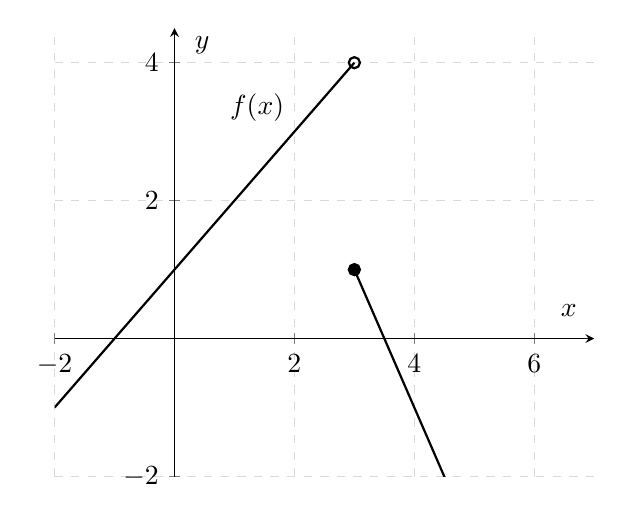
\begin{tikzpicture}
  \begin{axis}[
    axis lines=middle,
    xlabel={$x$}, ylabel={$y$},
    every axis x label/.style={at={(ticklabel* cs:0.92)}, anchor=west, yshift=10pt},
    every axis y label/.style={at={(ticklabel* cs:0.92)}, anchor=south, xshift=10pt},
    xmin=-2, xmax=7, ymin=-2, ymax=4.5,
    xtick={-2,0,2,4,6},
    ytick={-2,0,2,4},
    grid=both,
    grid style={dashed,gray!30},
  ]
    \addplot [domain=-2:3, thick] {x+1}
      node[above left,pos=0.8] {$f(x)$};
    \addplot [domain=3:7, thick] {-2*x+7};
    % open and closed points at x=3
    \addplot [only marks, mark=o, thick] coordinates {(3,4)};
    \addplot [only marks, mark=*, thick] coordinates {(3,1)};
  \end{axis}
\end{tikzpicture}\end{center}
 On observe que 
 \[\lim_{x\rightarrow 3^+}f(x)=\ligne{1} \quad \text{et} \quad \lim_{x\rightarrow 3^-}f(x)=\ligne{1}\]
 donc la limite $\displaystyle{\lim_{x\rightarrow 3}f(x)}$ \ligne{3}.
\end{exemple}
\begin{exemple}
	\tcblower
	Soit la fonction $f$ définie par $f(x)=\dfrac{9-x}{3-\sqrt{x}}$. Étudier graphiquement $\displaystyle{\lim_{x\rightarrow 9}f(x)}$ et $\displaystyle{\lim_{x\rightarrow 4}f(x)}$.

	Le domaine de définition de $f$ est 
	$D_f=\ligne{4}$. 
\begin{center}
	\begin{tikzpicture}[scale=0.8]
  \begin{axis}[
    axis lines=middle,
    xlabel={$x$}, ylabel={$y$},
    every axis x label/.style={at={(ticklabel* cs:0.92)}, anchor=west, yshift=10pt},
    every axis y label/.style={at={(ticklabel* cs:0.92)}, anchor=south, xshift=10pt},
    xmin=0,   xmax=15,
    ymin=0,   ymax=9,
    xtick={0,4,9,15},
    ytick={0,5,6,8},
    grid=both,
    grid style={dashed,gray!30},
  ]
    % branche pour 0 ≤ x < 9
    \addplot[domain=0:8.9, samples=200, thick]
      {(9 - x)/(3 - sqrt(x))};
    % branche pour x > 9
    \addplot[domain=9.1:15, samples=200, thick]
      {(9 - x)/(3 - sqrt(x))}
      node[above,pos=0.5] {$f(x)$};
    % point ouvert en (9,6)
    \addplot[only marks, mark=o, thick] coordinates {(9,6)};
    % point fermé en (4,5)
    \addplot[only marks, mark=*, thick] coordinates {(4,5)};
    % traits pointillés illustrant les limites/valeurs
    \draw[dashed] (axis cs:0,6) -- (axis cs:9,6);
    \draw[dashed] (axis cs:9,0) -- (axis cs:9,6);
    \draw[dashed] (axis cs:0,5) -- (axis cs:4,5);
    \draw[dashed] (axis cs:4,0) -- (axis cs:4,5);
  \end{axis}
\end{tikzpicture}
\end{center}
On a $\displaystyle{\lim_{x\rightarrow 9}f(x)=}\ligne{1}$ même si $f$ n'est pas définie en $9$ (indiqué par le rond vide). De plus $\displaystyle{\lim_{x\rightarrow 4}f(x)=}\ligne{1}$. On a calculé les deux limites et on a montré qu'elles \ligne{2}.  
\end{exemple}
\begin{exemple}
	\tcblower
	Soit $f$ définie par $f(x)=\dfrac{x^3-1}{x^2-1}$. Déterminer $\displaystyle{\lim_{x\rightarrow 1}f(x)}$ et $\displaystyle{\lim_{x\rightarrow -1}f(x)}$.

	On a $D_f=\mathbb{R}\setminus\{-1\}$. 
	\begin{center}
		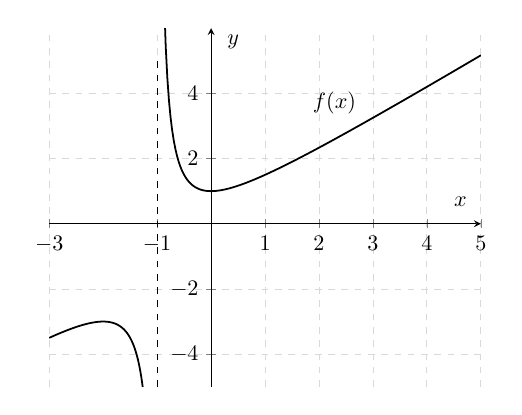
\begin{tikzpicture}[scale=0.8]
  \begin{axis}[
    axis lines=middle,
    every axis x label/.style={at={(ticklabel* cs:0.92)}, anchor=west, yshift=10pt},
    every axis y label/.style={at={(ticklabel* cs:0.92)}, anchor=south, xshift=10pt},
    xlabel={$x$}, ylabel={$y$},
    xmin=-3, xmax=5, ymin=-5, ymax=6,
    xtick={-3,-1,0,1,2,3,4,5},
    ytick={-4,-2,0,2,4},
    grid=both,
    grid style={dashed,gray!30},
  ]
    % branche pour x < -1
    \addplot [domain=-3:-1.1, samples=200, thick]
      {(x^3-1)/(x^2-1)};
    \addplot [domain=-0.9:5, samples=200, thick]
      {(x^3-1)/(x^2-1)} node[above left,pos=0.8] {$f(x)$};
    % asymptote verticale en x = -1
    \draw[dashed] (axis cs:-1,-5) -- (axis cs:-1,5);
  \end{axis}
\end{tikzpicture}
	\end{center}
	On observe que 
	\[\displaystyle{\lim_{x\rightarrow 1^-}f(x)=\dfrac{3}{2}} \quad \text{et} \quad \displaystyle{\lim_{x\rightarrow 1^+}f(x)=\dfrac{3}{2}}\]
	donc $\displaystyle{\lim_{x\rightarrow 1}f(x)}$ existe et vaut $\dfrac{3}{2}$. Toutefois, $\displaystyle{\lim_{x\rightarrow -1^-}f(x)=}\ligne{1}$ et 

$\displaystyle{\lim_{x\rightarrow -1^+}f(x)=}\ligne{1}$
donc $\displaystyle{\lim_{x\rightarrow -1}f(x)} \ligne{3}$.
\end{exemple} 

Il existe une définition plus formelle de la limite, mais elle sort du cadre de ce cours. Nous verrons dès la section \ref{sec:limel} des outils pour calculer plus rigoureusement des limites. Certains des résultats seront démontrés et d'autres seront acceptés sans démonstration.

\subsection{Lien avec la continuité}
On peut à présent donner une caractérisation plus formelle de la continuité. 

\begin{thm}
Continuité
	\tcblower
Soit $f : I \to \mathbb{R}$ une fonction réelle (donc $I \subset \mathbb{R}$) et $a \in I$.  
\medskip

\begin{minipage}[c][0.8cm]{0.5\textwidth}{
		\begin{center}
$f$ est continue en $a$ ssi  
\end{center}
}
\end{minipage}
\hfill
\begin{minipage}[c]{0.5\textwidth}{
\vspace{0pt}
\begin{enumerate}
\item $\displaystyle\lim_{x\to a}f(x)$ existe dans $\mathbb{R}$;
\item $f(a)$  existe dans $\mathbb{R}$;
\item $\displaystyle\lim_{x\to a}f(x)=f(a)$.
\end{enumerate}
}
\end{minipage}
\medskip

Pour être plus concis, on écrira simplement :  
\[f \text{ est continue en }a \Longleftrightarrow \displaystyle\lim_{x\to a}f(x)=f(a).\]
\end{thm}
\begin{remarque}
	\tcblower
	On peut également écrire
	\[f \text{ est continue en }x \Longleftrightarrow \displaystyle\lim_{h\to 0}f(x+h)=f(x).\]
\end{remarque}
Reprenons l'exemple \ref{ex:continuiteintro} avec ce résultat.
\begin{exemple}
	\tcblower
	\begin{tasks}(2)
	\task 

	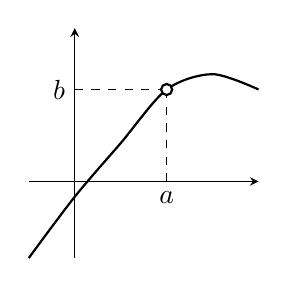
\begin{tikzpicture}[>=stealth]
% ------------------------------------------------------------------
% 1 ── no value at a (open circle)
\begin{axis}[
    name=G1,
    width=4.5cm,height=4.5cm,
    axis lines=middle, axis line style={->},
    xmin=-1,xmax=4, ymin=-1,ymax=2,
    xtick=\empty, ytick=\empty,
    clip=false]
  \addplot[smooth,thick] coordinates
      {(-1,-1) (0,-0.2) (1,0.5) (2,1.2) (3,1.4) (4,1.2)};
  \draw[dashed] (axis cs:2,0) -- (axis cs:2,1.2);
  \draw[dashed] (axis cs:0,1.2) -- (axis cs:2,1.2);
  \draw[fill=white,thick] (axis cs:2,1.2) circle (2pt); % ∘
  \node[below] at (axis cs:2,0) {$a$};
  \node[left]  at (axis cs:0,1.2) {$b$};
\end{axis}
\end{tikzpicture}

$f$ n'est pas continue en $a$, car $f$ n'est pas définie en $a$.
\task 




\begin{tikzpicture}[>=stealth]

	% ------------------------------------------------------------------
% 2 ── continuous, piecewise-linear peak
\begin{axis}[
    at={(G1.east)}, xshift=1.5cm,
    width=4.5cm,height=4.5cm,
    axis lines=middle, axis line style={->},
    xmin=-1,xmax=5, ymin=-1,ymax=2,
    xtick=\empty, ytick=\empty,
    clip=false]
  \addplot[thick] coordinates {(-1,-0.3) (2,1.4) (5,-0.6)};
  \draw[dashed] (axis cs:2,0) -- (axis cs:2,1.4);
  \draw[dashed] (axis cs:-0.1,1.4) -- (axis cs:2,1.4);
  \draw[fill=black] (axis cs:2,1.4) circle (2pt);
  \node[below] at (axis cs:2,0) {$a$};
  \node[left]  at (axis cs:0,1.4) {$b$};
\end{axis}
\end{tikzpicture}

$f$ est continue en $a$, car 

$\displaystyle{\lim_{x\rightarrow a}f(x)=f(a)=b}$ 

\task 

\begin{tikzpicture}[>=stealth]
	\begin{axis}[
    at={(G1 -| G1.east)}, xshift=3cm,
    width=4.5cm,height=4.5cm,
    axis lines=middle, axis line style={->},
    xmin=-1,xmax=4, ymin=-1,ymax=2,
    xtick=\empty, ytick=\empty,
    clip=false]
  \addplot[smooth,thick,domain=-1:2,samples=80] {0.6+0.5*x-0.2*x^2};
  \addplot[smooth,thick,domain=2:4,samples=80] {0.06*(x-2)^2+0.15*(x-2)+0};
  % points & guides
  \draw[dashed] (axis cs:2,0) -- (axis cs:2,0.8);
  \draw[dashed] (axis cs:0,0.8) -- (axis cs:2,0.8);
  \draw[dashed] (axis cs:0,0) -- (axis cs:2,0);
  \draw[fill=white,thick] (axis cs:2,0) circle (2pt);   % open
  \draw[fill=black]       (axis cs:2,0.8) circle (2pt); % closed
  \node[below] at (axis cs:2,0) {$a$};
  \node[left]  at (axis cs:0,0.8) {$b$};
\end{axis}
\end{tikzpicture}

$f$ n'est pas continue en $a$, car

$\displaystyle{\lim_{x\rightarrow a}f(x)}$ n'existe pas. 

\task 

\begin{tikzpicture}[>=stealth]
	\begin{axis}[
    at={(G1.south)}, yshift=-1.5cm,
    width=4.5cm,height=4.5cm,
    axis lines=middle, axis line style={->},
    xmin=-1,xmax=4, ymin=-1,ymax=2,
    xtick=\empty, ytick=\empty,
    clip=false]
  \addplot[smooth,thick,domain=-1:4,samples=100]
      {-0.25*(x-2)^2+1.2};
  \draw[dashed] (axis cs:2,0) -- (axis cs:2,1.2);
  \draw[dashed] (axis cs:0,1.2) -- (axis cs:2,1.2);
  \draw[dashed] (axis cs:0,0.5) -- (axis cs:2,0.5);
  \draw[dashed] (axis cs:0,0.0) -- (axis cs:2,0.0);
  \draw[fill=white,thick] (axis cs:2,1.2) circle (2pt); % open
  \draw[fill=black]       (axis cs:2,0.5) circle (2pt); % value
  \node[below] at (axis cs:2,0) {$a$};
  \node[left]  at (axis cs:0,1.2) {$b$};
  \node[left]  at (axis cs:0,0.5) {$c$};
\end{axis}
\end{tikzpicture}

$f$ n'est pas continue en $a$, car

$\displaystyle{\lim_{x\rightarrow a}f(x)=b\neq f(a)=c}$. 

		\task[e)] 

\begin{tikzpicture}[>=stealth]
	\begin{axis}[
    at={(G1 -| G1.east |- G1.south)}, xshift=3cm,
    width=4.5cm,height=4.5cm,
    axis lines=middle, axis line style={->},
    xmin=-1,xmax=4, ymin=-1,ymax=2,
    xtick=\empty, ytick=\empty,
    clip=false]
  \addplot[smooth,thick,domain=-1:4,samples=100] {0.1*(x-2)^3 -0.5*(x-2) +0.3};
  \draw[dashed] (axis cs:2,0.3) -- (axis cs:0,0.3);
  \draw[dashed] (axis cs:2,0) -- (axis cs:2,0.3);
  \draw[fill=black] (axis cs:2,0.3) circle (2pt);
  \node[below] at (axis cs:2,0) {$a$};
  \node[above left]  at (axis cs:0,0.3) {$b$};
\end{axis}
\end{tikzpicture}

$f$ est continue en $a$, car 

$\displaystyle{\lim_{x\rightarrow a}f(x)=f(a)=b}.$ 

\task[f)] 

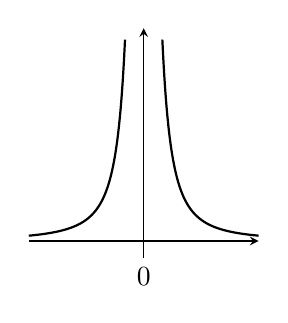
\begin{tikzpicture}[>=stealth]
\begin{axis}[
    width=4.5cm,height=4.5cm,
    axis lines=middle, axis line style={->},
    xmin=-4,xmax=4, ymin=-0.2,ymax=2.5,
    xtick=\empty, ytick=\empty,
    clip=false]
  % 1/x² left branch
  \addplot[domain=-4:-0.65,samples=200,thick] {1/(x^2)};
  % 1/x² right branch
  \addplot[domain=0.65:4,samples=200,thick] {1/(x^2)};
  % vertical asymptote x = 0
  \draw[dashed] (axis cs:0,-0.2) -- (axis cs:0,2.5);
  \node[below] at (axis cs:0,-0.2) {$0$};
\end{axis}
\end{tikzpicture}

$f$ n'est pas continue en $0$, car

$\displaystyle{\lim_{x\rightarrow 0}f(x)=+\infty}$. 

	\end{tasks}
\end{exemple}

\begin{definition}
	continuité à gauche\\
	continuité à droite
	\tcblower
	Soit $f: I\rightarrow \mathbb{R}$ une fonction réelle et $a\in I$.

	\[f \text{ est continue à gauche en } a \text{ ssi } \displaystyle{\lim_{x\rightarrow a^-}f(x)=f(a)}\]
	\[f \text{ est continue à droite en } a \text{ ssi } \displaystyle{\lim_{x\rightarrow a^+}f(x)=f(a)}\]
\end{definition}
\begin{exemple}
	\tcblower
	\begin{minipage}[t]{0.55\textwidth}{
	\vspace{0pt}
$f$ est continue à gauche, car $\displaystyle{\lim_{x\rightarrow a^-}f(x)=f(a)=b}$

\medskip
$f$ n'est pas continue à droite, car $\displaystyle{\lim_{x\rightarrow a^+}f(x)\neq f(a)=b}$.  	
	}
	\end{minipage}
	\begin{minipage}[t]{0.4\textwidth}{
	\vspace{0pt}
	\begin{center}
\begin{tikzpicture}[>=stealth]
	\begin{axis}[
    at={(G1 -| G1.east)}, xshift=3cm,
    width=5.5cm,height=5.5cm,
    axis lines=middle, axis line style={->},
    xmin=-1,xmax=4, ymin=-1,ymax=2,
    xtick=\empty, ytick=\empty,
    clip=false]
  \addplot[smooth,thick,domain=-1:2,samples=80] {0.6+0.5*x-0.2*x^2};
  \addplot[smooth,thick,domain=2:4,samples=80] {0.06*(x-2)^2+0.15*(x-2)+0};
  % points & guides
  \draw[dashed] (axis cs:2,0) -- (axis cs:2,0.8);
  \draw[dashed] (axis cs:0,0.8) -- (axis cs:2,0.8);
  \draw[dashed] (axis cs:0,0) -- (axis cs:2,0);
  \draw[fill=white,thick] (axis cs:2,0) circle (2pt);   % open
  \draw[fill=black]       (axis cs:2,0.8) circle (2pt); % closed
  \node[below] at (axis cs:2,0) {$a$};
  \node[left]  at (axis cs:0,0.8) {$b$};
\end{axis}
\end{tikzpicture}

	\end{center}
	}
	\end{minipage}
\end{exemple}



\subsection{Limite de fonctions élémentaires}
\label{sec:limel}
\begin{thm}[label=thm:limel]
Limites de fonctions élémentaires

(sans démonstration)
	\tcblower
	\noindent\begin{description}
		\item[{\bfseries L1}] Si $k\in\mathbb{R}$, alors $\displaystyle{\lim_{x\rightarrow a}k=k}, \,\forall a\in\mathbb{R}$
		\item[{\bfseries L2}] Si $x\in \mathbb{R}$, alors $\displaystyle{\lim_{x\rightarrow a}x=a}, \,\forall a\in \mathbb{R}$
		\item[{\bfseries L3}] Si $x\in \mathbb{R}$, alors $\displaystyle{\lim_{x\rightarrow a}\sin(x)=\sin(a)}$ et $\displaystyle{\lim_{x\rightarrow a}\cos(x)=\cos(a)},\, \forall a\in \mathbb{R}$
		\item[{\bfseries L4}] Si $f(x)=\sqrt[n]{x}$ et $D_f$ est son domaine de définition, 

			alors $\displaystyle{\lim_{x\rightarrow a}\sqrt[n]{x}=\sqrt[n]{a}}, \, \forall a \in D_f$ 
		\item[{\bfseries L5}] Si $b\in \mathbb{R}_{>0}\setminus\{1\}$, alors $\displaystyle{\lim_{x\rightarrow a}\log_b(x)=\log_b(a)}, \,\forall a\in \mathbb{R}_{>0}$ et 

			$\displaystyle{\lim_{x\rightarrow a}\exp_b(x)=\exp_b(a)},\,\forall a\in \mathbb{R}$  	
	\end{description}
\end{thm}
\begin{exemple}
	\tcblower
	$\displaystyle{\lim_{x\rightarrow -3}14\stackrel{\text{\eqmakebox[b][c]{{\bfseries L1}}}}{=}14}$, par la première assertion du théorème \ref{thm:limel}. 
\end{exemple}

\begin{exemple}
	\tcblower
$\displaystyle{\lim_{x\rightarrow 5}x\stackrel{\text{\eqmakebox[b][c]{{\bfseries L2}}}}{=}5}$ 
\end{exemple}

\begin{exemple}
	\tcblower
	$\displaystyle{\lim_{x\rightarrow \pi/2}\sin(x)\stackrel{\text{\eqmakebox[b][c]{{\bfseries L3}}}}{=}\sin\left(\dfrac{\pi}{2}\right)}=1$ 
\end{exemple}
\begin{exemple}
	\tcblower
	$\displaystyle{\lim_{x\rightarrow 8}\sqrt[3]{x}\stackrel{\text{\eqmakebox[b][c]{{\bfseries L4}}}}{=}\sqrt[3]{8}=2}$ 
\end{exemple}


\begin{coro}
	Fonctions continues
	\tcblower
	\noindent\begin{description}
		\item[{\bfseries C1}] Les fonctions constantes sont continues sur $\mathbb{R}$.  
		\item[{\bfseries C2}] La fonction $f$ définie par $f(x)=x$ est continue sur $\mathbb{R}$.  
		\item[{\bfseries C3}] Les fonctions $\sin$ et $\cos$ sont continues sur $\mathbb{R}$. 
		\item[{\bfseries C4}] Les fonctions racines-n-ièmes sont continues sur leur domaine de définition.
		\item[{\bfseries C5}] Les fonctions exponentielles et logarithmes sont continues sur leur domaine de définition. 
	\end{description}
\end{coro}


\subsection{Propriétés des limites}
\label{sec:proplim}
Les propriétés suivantes nous permettent de calculer des limites plus compliquées du type $\displaystyle{\lim_{x\rightarrow 2}\dfrac{x-5}{x}}$.
\smallskip
\begin{thm}[label=thm:limprop]
	Propriétés des limites

	(sans démonstration)
	\tcblower
Si $\displaystyle{\lim_{x\rightarrow a}f(x)}$ et $\displaystyle{\lim_{x\rightarrow a}g(x)}$ existent et sont finies, alors on a 
\noindent
\begin{description}
	\item[{\bfseries P0}] $\displaystyle{\lim_{x\rightarrow a}k\cdot f(x)=k\cdot \lim_{x\rightarrow a}f(x)},\, \forall k\in \mathbb{R}$ 
	\item[{\bfseries P1}] $\displaystyle{\lim_{x\rightarrow a}\left(f(x)+g(x)\right)=\lim_{x\rightarrow a}f(x)+\lim_{x\rightarrow a}g(x)}$ 
	\item[{\bfseries P2}] $\displaystyle{\lim_{x\rightarrow a}\left(f(x)-g(x)\right)=\lim_{x\rightarrow a}f(x)-\lim_{x\rightarrow a}g(x)}$ 
	\item[{\bfseries P3}] $\displaystyle{\lim_{x\rightarrow a}\left(f(x)\cdot g(x)\right)=\lim_{x\rightarrow a}f(x)\cdot \lim_{x\rightarrow a}g(x)}$ 
	\item[{\bfseries P4}] $\displaystyle{\lim_{x\rightarrow a}\dfrac{f(x)}{g(x)}=\dfrac{\lim_{x\rightarrow a}f(x)}{\lim_{x\rightarrow a}g(x)}}$ 
\end{description}
\end{thm}
\begin{thm}[label=thm:compo]
	Limite d'une composition

	(sans démonstration)
	\tcblower
	Si $\displaystyle{\lim_{x\rightarrow a}f(x)=b}$ et $\displaystyle{\lim_{t\rightarrow b}g(t)=g(b)}$ existent et sont finies, alors on a~:
	\[\lim_{x\rightarrow a}g(f(x))=g(\lim_{x\rightarrow a }f(x))=g(b).\] 
\end{thm}
\begin{coro}
Opérations de

fonctions continues
	\tcblower
	\noindent\begin{description}
		\item[{\bfseries PC1}] Si $f$ est $g$ sont continues en $a$, alors $f+g$ est continue en $a$.  
		\item[{\bfseries PC2}] Si $f$ est $g$ sont continues en $a$, alors $f-g$ est continue en $a$.  
		\item[{\bfseries PC3}] Si $f$ est $g$ sont continues en $a$, alors $f\cdot g$ est continue en $a$.  
		\item[{\bfseries PC4}] Si $f$ est $g$ sont continues en $a$ et $g(a)\neq 0$, alors $\dfrac{f}{g}$ est continue en $a$.  
		\item[{\bfseries PC5}] Si $f$ est continue en $a$ et $g$ est continue en $f(a)$, alors $g\circ f$ est continue en $a$. 
	\end{description}
\end{coro}

\begin{coro}[label=thm:poly]
Limites de fonctions polynômiales	

(avec démonstration)
	\tcblower
	Si $f$ est une fonction polynomiale, i.e. 
	\[f(x)=a_nx^n+a_{n-1}x^{n-1}+\ldots+a_2 x^2+a_1x_1+a_0,\]
	alors, pour $b\in\mathbb{R}$, on a~:
	\[\lim_{x\rightarrow b}f(x)=f(b)=a_n b^n+\ldots+a_1b+a_0.\]
\begin{proof}
	On a $\displaystyle{\lim_{x\rightarrow b}x}\stackrel{\text{\eqmakebox[b][c]{{\bfseries L2}}}}{=}b$. De plus, pour tout $m\in \mathbb{N}$, 

	\[\displaystyle{\lim_{x\rightarrow b}x^m\stackrel{\text{\eqmakebox[b][c]{\bfseries P3}}}{=}}\left(\displaystyle{\lim_{x\rightarrow b}x}\right)^m=b^m.\] 

Ainsi,
\begin{align*}
	\lim_{x\rightarrow b} \left(a_nx^n+\ldots +a_1x_1+a_0\right)&\stackrel{\text{\eqmakebox[c][c]{{\bfseries P1}}}}{=}\lim_{x\rightarrow b} a_nx^n+\ldots+\lim_{x\rightarrow b} a_1x+\lim_{x\rightarrow b}a_0\\
									     &\stackrel{\text{\eqmakebox[c][c]{{\bfseries P0}}}}{=}a_n\lim_{x\rightarrow b} x^n+\ldots+a_1\cdot\lim_{x\rightarrow b} x+a_0\\							     
									     &\stackrel{\text{\eqmakebox[c][c]{{\bfseries P3 et L2}}}}{=}a_n b^n+\ldots+a_1b+a_0.
\end{align*}


\end{proof}
\end{coro}



\begin{exemple}
	\tcblower
On peut maintenant calculer la limite considérée en introduction en justifiant le calcul :
	\[\lim_{x\to2}\left(\dfrac{x-5}{x}\right)
		\stackrel{\text{\eqmakebox[k][c]{{\bfseries P4}}}}{=}
\dfrac{\displaystyle{\lim_{x\to2}(x-5)}}{\displaystyle{\lim_{x\to2}x}}
\stackrel{\text{\eqmakebox[k][c]{{\bfseries {P2}}}}}{=}
\dfrac{\displaystyle{\lim_{x\to2}x-\lim_{x\to2}5}}{\displaystyle{\lim_{x\to2}x}}
\stackrel{\text{{\eqmakebox[k][c]{\bfseries {L2,L1}}}}}{=}
\dfrac{2-5}{2}
=-\dfrac{3}{2}
\]
\end{exemple}


\begin{exemple}
	\tcblower
Calculer en justifiant 
\begin{tasks}
	\task
\[
\lim_{x\to-4}(x+3)
\stackrel{\text{\eqmakebox[l][c]{{\bfseries{P1}}}}}{=}
\lim_{x\to-4}x+\lim_{x\to-4}3
\stackrel{\text{\eqmakebox[l][c]{{\bfseries{L2,L1}}}}}{=}
-4+3=-1
\]
ou plus directement :
\[
\lim_{x\to-4}(x+3)
\stackrel{\text{\eqmakebox[l][c]{{\bfseries{thm \ref{thm:poly}}}}}}{=}
-4+3=-1
\]


\task 

\[
\lim_{x\to1}2x^2
\stackrel{\text{\eqmakebox[m][c]{{\bfseries{P0}}}}}{=}
2\cdot\lim_{x\to1}x^2
\stackrel{\text{\eqmakebox[m][c]{{\bfseries{P3}}}}}{=}
2\cdot\lim_{x\to1}x\cdot\lim_{x\to1}x
\stackrel{\text{\eqmakebox[m][c]{{\bfseries{L2,L1}}}}}{=}
2\cdot1\cdot1=2
\]
ou plus directement :
\[
\lim_{x\to1}2x^2
\stackrel{\text{\eqmakebox[m][c]{{\bfseries{thm \ref{thm:poly}}}}}}{=}
2\cdot1\cdot1=2
\]
\end{tasks}
\end{exemple}
\begin{exemplesuite}
\tcblower
	\begin{tasks}
		\task[c)]
\[
\lim_{x\to2}\dfrac{x+5}{x}
\stackrel{\text{\eqmakebox[b][c]{{\bfseries{P4}}}}}{=}
\dfrac{\lim_{x\to2}(x+5)}{\lim_{x\to2}x}
\stackrel{\text{\eqmakebox[m][c]{{\bfseries thm. \ref{thm:poly}}}}}{=}
\dfrac{2+5}{2}
=\dfrac{7}{2}
\]
\task[d)]
\[
\lim_{x\to0}\cos(x^4)
\stackrel{\text{\eqmakebox[d][c]{{\bfseries{L3 et thm \ref{thm:compo}}}}}}{=}
\cos\bigl(\lim_{x\to0}x^4\bigr)
\stackrel{\text{\eqmakebox[m][c]{{\bfseries thm \ref{thm:poly}}}}}{=}
\cos(0^4)=\cos(0)=1
\]
\end{tasks}
\end{exemplesuite}
\begin{thm}
	(sans démonstration)
	\tcblower
	Soient $f$ et $g$ deux fonctions définies sur un voisinage $I$ de $a\in \mathbb{R}$ telles que  
	\begin{tasks}
		\task $f(x)\leq g(x),\, \forall x \in I$
		\task $\displaystyle{\lim_{x\rightarrow a}f(x)}$ et $\displaystyle{\lim_{x\rightarrow a}g(x)}$ existent  
	\end{tasks} alors 

	\[\displaystyle{\lim_{x\rightarrow a}f(x)}\leq  \displaystyle{\lim_{x\rightarrow a}g(x)}, \forall a\in I\]

	%($a$ peut également valoir $-\infty$ et $+\infty$ si l'intervalle $I$ n'est pas borné).
\end{thm}
\begin{thm}
	Théorème des gendarmes
	(sans démonstration)
	\tcblower
	Soient $f, g$ et $h$ des fonctions définies sur un voisinage $I$ de $a\in \mathbb{R}$ %($a$ peut également valoir $-\infty$ ou $+\infty$) 
	telles que
	\begin{tasks}
		\task $f(x)\leq g(x)\leq h(x),\, \forall x \in I\setminus\{a\}$
		\task $\displaystyle{\lim_{x\rightarrow a}f(x)}=\displaystyle{\lim_{x\rightarrow a}h(x)}=\ell\in \mathbb{R}$ 

		%($\ell$ peut également être égal au symbole $-\infty$ ou $+\infty$).  
	\end{tasks} alors 

	\[\displaystyle{\lim_{x\rightarrow a}g(x)}=\ell.\]
\end{thm}
\begin{coro}
(avec démonstration)
	\tcblower 
	La fonction $f(x)=\begin{cases}x\sin\left(\dfrac{1}{x}\right),& x\neq 0\\
	0, &x=0\end{cases}$ est continue.

	\begin{proof}
Voir les exercices. 
	\end{proof}
	
\end{coro}
\subsection{Limites infinies -- types « $\dfrac{1}{0}$ » et « $\dfrac{0}{0}$ »}
\begin{definition}
	Type $«~\dfrac{1}{0}~»$
	\tcblower
	Une limite du type quotient \(\displaystyle \lim_{x\to a}\dfrac{f(x)}{g(x)}\) pour laquelle on a \(\displaystyle \lim_{x\to a}g(x)=0\) mais où \(\displaystyle \lim_{x\to a}f(x)\neq0\) est appelée limite de type \(«~\displaystyle \dfrac{1}{0}~»\). 
\end{definition}
\begin{remarque}
	\tcblower
	Il y a deux cas pour les limites «~$\dfrac{1}{0}$~»~:
	\begin{description}
		\item[Cas 1] La limite existe et vaut $-\infty$ ou $+\infty$.
		\item[Cas 2] La limite n'existe pas, (par exemple, limite à gauche vaut $-\infty$ et limite à droite vaut $+\infty$.).
	\end{description}
	{\bfseries Conclusion~:} Il faut calculer la limite à gauche et à droite en s'aidant, si besoin, de la factorisation.
\end{remarque}


\begin{exemple}
\begin{tikzpicture}[scale=0.5]
  \begin{axis}[
    axis lines=middle,
    xlabel={}, ylabel={},
    xlabel style={at=(current axis.right of origin), anchor=west},
    ylabel style={at=(current axis.above origin), anchor=south},
    xmin=-3, xmax=3, ymin=-4, ymax=4,
    xtick={-3,-2,-1,1,2,3},
    ytick={-4,-2,2,4},
      yticklabel=\empty,
      xticklabel=\empty,
    %grid=both,
    grid style={dashed,gray!30},
  ]
    % branches of 1/x
    \addplot [domain=-3:-0.1,samples=200, thick] {1/x};
    \addplot [domain=0.1:3, samples=200, thick] {1/x}
      node[above right,pos=0.8] {$f(x)=\dfrac1x$};
    % asymptotes
    \draw[dashed] (axis cs:0,-4) -- (axis cs:0,4);
    \draw[dashed] (axis cs:-3,0) -- (axis cs:5,0);
  \end{axis}
\end{tikzpicture}
	\tcblower


Soit \(f\) définie par \(f(x)=\dfrac1x\) : $\lim_{x\to0^-}\dfrac1x
=«\dfrac{1}{0^-}»=\ligne{1}$, 
\[
\lim_{x\to0^+}\dfrac1x
=«\dfrac{1}{0^+}»=\ligne{1}, \text{donc } \displaystyle \lim_{x\to0}\dfrac1x
\,\ligne{3}\]
\end{exemple}
\begin{exemple}
% f(x) = 1/x^2
\begin{tikzpicture}[scale=0.5]
  \begin{axis}[
    axis lines=middle,
    xlabel={}, ylabel={},
    xlabel style={at=(current axis.right of origin), anchor=west},
    ylabel style={at=(current axis.above origin), anchor=south},
    xmin=-3, xmax=3, ymin=-2, ymax=4,
    xtick={-3,-2,-1,1,2,3},
    ytick={-2,2,4},
      yticklabel=\empty,
      xticklabel=\empty,
    %grid=both,
    grid style={dashed,gray!30},
  ]
    % branches of 1/x
    \addplot [domain=-3:-0.1,samples=200, thick] {1/(x*x)};
    \addplot [domain=0.1:3, samples=200, thick] {1/(x*x)}
	    node[above left,pos=1] {$f(x)=\dfrac{1}{x^2}$};
    % asymptotes
    \draw[dashed] (axis cs:0,-4) -- (axis cs:0,4);
    \draw[dashed] (axis cs:-3,0) -- (axis cs:5,0);
  \end{axis}
\end{tikzpicture}	\tcblower

Soit \(f\) définie par \(f(x)=\dfrac1{x^2}\) :$\lim_{x\to0^-}\dfrac1{x^2}=« \dfrac{1}{(0^-)^2} »=\ligne{1},$ 
\[
\lim_{x\to0^+}\dfrac1{x^2}
=«\dfrac{1}{(0^+)^2}»=\ligne{1}, \text{donc } \displaystyle\lim_{x\to0}\dfrac1{x^2}=\ligne{1}.\]
\end{exemple}


\begin{exemple}[label=ex:inf1]
	\tcblower
Calculer  \(\displaystyle\lim_{x\to -2}\dfrac{-2}{2x+4}\) et interpréter graphiquement.
\[
\lim_{x\to -2}\dfrac{-2}{2x+4}
=«~\dfrac{-2}{0}~»
\,: \text{c'est un type }«~\dfrac{1}{0}~»;
\]
\[
\lim_{x\to -2^+}\dfrac{-2}{2x+4}
=\lim_{x\to -2^+}\dfrac{-2}{2(x+2)}
=\lim_{x\to -2^+}\dfrac{-1}{x+2}
=«~\dfrac{-1}{0^+}~»
=\ligne{1},
\]
et
\[
\lim_{x\to -2^-}\dfrac{-2}{2x+4}
=«~\dfrac{-1}{0^-}~»
=\ligne{1} \text{ d'où } \displaystyle{\lim_{x\to -2}\dfrac{-2}{2x+4}}\, \ligne{3}.\] 
\end{exemple}
\begin{exemple}[label=ex:inf2]
	Calculer  \(\displaystyle\lim_{x\to -2}\dfrac{-2}{(x+2)^2}\) et interpréter graphiquement.
	\tcblower
\[
\lim_{x\to -2}\dfrac{-2}{(x+2)^2}
=«~\dfrac{-2}{0}~»
\,: \text{c'est un type }«~\dfrac{1}{0}~»
;
\]
\[
\lim_{x\to -2^-}\dfrac{-2}{(x+2)^2}
=«~\dfrac{-2}{(0^-)^2~»
}
=\ligne{1} \text{ et } 
\lim_{x\to -2^+}\dfrac{-2}{(x+2)^2}
=«~\dfrac{-2}{(0^+)^2~»
}
=\ligne{1},
\]
donc $\displaystyle\lim_{x\to -2}\dfrac{-2}{(x+2)^2}\ligne{2}$.
\end{exemple}
\begin{exemple}[label=ex:inf3]
	Calculer \(\displaystyle\lim_{x\to 1}\dfrac{x-2}{x^2+3x-4}\) et interpréter graphiquement.
	\tcblower
\[
\lim_{x\to 1}\dfrac{x-2}{x^2+3x-4}
=«~\dfrac{-1}{0}~»
\,: \text{c'est un type }«~\dfrac{1}{0}~»
;
\]
\[
\lim_{x\to 1^+}\dfrac{x-2}{x^2+3x-4}
=\lim_{x\to 1^+}\dfrac{x-2}{(x-1)(x+4)}
=«~\dfrac{-1}{0^+\cdot5}~»
=\ligne{1}\]
et
\vspace{-0.3cm}
\[
\lim_{x\to 1^-}\dfrac{x-2}{x^2+3x-4}
=\lim_{x\to 1^-}\dfrac{x-2}{(x-1)(x+4)}
=«~\dfrac{-1}{0^-\cdot5}~»
=\ligne{1},
\]
donc $\displaystyle\lim_{x\to 1}\dfrac{x-2}{x^2+3x-4}\,\ligne{3}$.
\end{exemple}

Interprétations graphiques :
\begin{center}
	\begin{tikzpicture}[scale=0.7]
    \begin{axis}[
	    axis lines=middle, xlabel={}, ylabel={},
      xmin=-5, xmax=1, ymin=-7, ymax=7,
      samples=200
    ]
    \node[anchor=north west] at (rel axis cs:0,1) {\bfseries Exemple \ref{ex:inf1}};
      \addplot[domain=-5:-2.1] {-2/(2*x+4)};
      \addplot[domain=-1.9:1]  {-2/(2*x+4)};
      \addplot[dashed] coordinates {(-2,-10) (-2,10)};
    \end{axis}
  \end{tikzpicture}
  \begin{tikzpicture}[scale=0.7]
    \begin{axis}[
      axis lines=middle,  xlabel={}, ylabel={},
      xmin=-5, xmax=1, ymin=-7, ymax=7,
      samples=200
    ]    \node[anchor=north west] at (rel axis cs:0,1) {\bfseries Exemple \ref{ex:inf2}};
      \addplot[domain=-5:-2.1] {-2/((x+2)^2)};
      \addplot[domain=-1.9:1]  {-2/((x+2)^2)};
      \addplot[dashed] coordinates {(-2,-10) (-2,10)};
    \end{axis}
  \end{tikzpicture}
  \begin{tikzpicture}[scale=0.7]
    \begin{axis}[
	    axis lines=middle, xlabel={}, ylabel={},
      xmin=-2, xmax=3, ymin=-7, ymax=7,
      samples=200
    ]    \node[anchor=north west] at (rel axis cs:0,1) {\bfseries Exemple \ref{ex:inf3}};
      \addplot[domain=-2:0.97]  {(x-2)/(x^2+3*x-4)};
      \addplot[domain=1.03:5]   {(x-2)/(x^2+3*x-4)};
      \addplot[dashed] coordinates {(1,-10) (1,10)};
    \end{axis}
  \end{tikzpicture}
\end{center}

\begin{definition}
	Type $«~\dfrac{0}{0}~»$
	\tcblower
	Une limite du type quotient \(\displaystyle \lim_{x\to a}\dfrac{f(x)}{g(x)}\) pour laquelle on a \(\displaystyle \lim_{x\to a}f(x)=0\) et \(\displaystyle \lim_{x\to a}g(x)=0\) est appelée limite de type \(«~\displaystyle \dfrac{0}{0}~»\). 
\end{definition}
\begin{remarque}
	\tcblower
Il y a trois cas pour les limites « $\dfrac{0}{0}$ »~:
\begin{description}
	\item[Cas 1] La limite existe et est finie.
	\item[Cas 2] La limite existe est est infinie.
	\item[Cas 3] La limite n'existe pas.
\end{description}
Il faut donc calculer la limite à droite et la limite à gauche à l'aide d'outils algébriques pour pouvoir {\bfseries lever l'indétermination}.
\end{remarque}

\begin{methode}
	Type $«~\dfrac{0}{0}~»$ polynomial
	\tcblower
Une limite \(\displaystyle\lim_{x\to a}\dfrac{f(x)}{g(x)}\) de type \(\displaystyle\dfrac{0}{0}\) où \(f(x)\) et \(g(x)\) sont des polynômes peut se calculer ainsi :
\begin{tasks}
	\task factoriser le numérateur et le dénominateur ;
	\task simplifier ; 
	\task si la nouvelle limite n’est plus du type «  \(\displaystyle\dfrac{0}{0}\) », la déterminer avec les outils connus.
\end{tasks}
\end{methode}
\begin{exemple}
\tcblower

\[
\lim_{x\to2}\dfrac{x^2-3x+2}{x^2-4}
=«~\dfrac{0}{0}~»\]
est du type $«~\dfrac{0}{0}~»$ avec polynômes au numérateur et au dénominateur. On procède de la sorte~:

$
\begin{aligned}
\lim_{x\to2}\dfrac{x^2-3x+2}{x^2-4}
&\stackrel{\text{\eqmakebox[a][c]{{\bfseries factoriser}}}}{=}
\lim_{x\to2}\dfrac{(x-2)(x-1)}{(x-2)(x+2)}\\
&\stackrel{\eqmakebox[a][c]{$x\neq2$}}{=}
\lim_{x\to2}\dfrac{x-1}{x+2}\\
&\stackrel{\text{\eqmakebox[a][c]{{\bfseries P4}}}}{=}
		  \displaystyle{		  \dfrac{\displaystyle{\lim_{x\to2}(x-1)}}{\displaystyle{\lim_{x\to2}(x+2)}}}\\
&\stackrel{\text{\eqmakebox[a][c]{{\bfseries thm \ref{thm:poly}}}}}{=}
\dfrac{1}{4}
\end{aligned}$
\end{exemple}

\begin{methode}
	Type $«~\dfrac{0}{0}~»$ racine carrée
	\tcblower
Une limite \(\displaystyle\lim_{x\to a}\dfrac{f(x)}{g(x)}\) de type \(\displaystyle\dfrac{0}{0}\) où \(f(x)\) et/ou \(g(x)\) contient une racine carrée peut se calculer ainsi :
\begin{tasks}
\task multiplier par le conjugué ;
\task développer l'expression \((a - b)(a + b)\) en \(a^2 - b^2\) avec la 3\textsuperscript{e} identité remarquable ;
\task simplifier ;
\task  si la nouvelle limite n’est plus du type \(\displaystyle\dfrac{0}{0}\), la déterminer avec les outils connus.
\end{tasks}
\end{methode}

\begin{exemple}
\tcblower
\[
\lim_{x\to9}\dfrac{\sqrt{x}-3}{x-9}
=«~\dfrac{0}{0}~»\]
est du type $«~\dfrac{0}{0}~»$ avec une racine carrée.

$
\begin{aligned}
	\displaystyle{\lim_{x\to9}\dfrac{\sqrt{x}-3}{x-9}}
&\stackrel{\text{\eqmakebox[a][c]{\bfseries mult. conj.}}}{=}
\displaystyle{\lim_{x\to9}\dfrac{(\sqrt{x}-3)(\sqrt{x}+3)}{(x-9)(\sqrt{x}+3)}}\\
&\stackrel{\eqmakebox[a][c]{{$x\neq9$}}}{=}
\displaystyle{\lim_{x\to9}\dfrac{x-9}{(x-9)(\sqrt{x}+3)}}\\
&\stackrel{\text{\eqmakebox[a][c]{{\bfseries P4 et thm \ref{thm:compo}}}}}{=}
\displaystyle{\lim_{x\to9}\dfrac{1}{\sqrt{x}+3}}\\
&\stackrel{\eqmakebox[a][c]{}}{=}
\dfrac{1}{\sqrt{9}+3}\\
&\stackrel{\eqmakebox[a][c]{}}{=}\dfrac{1}{6}
\end{aligned}
$
\end{exemple}


\subsection{Asymptotes verticales}
\begin{definition}
	asymptote
	verticale
	\tcblower
On dit qu'une droite verticale d'équation $x = a$ est une \textbf{asymptote verticale} de la fonction $f$ ssi au moins l'une des conditions suivantes est satisfaite~:

$\displaystyle\lim_{x \to a^+} f(x) = +\infty$,  $\displaystyle\lim_{x \to a^+} f(x) = -\infty$,  $\displaystyle\lim_{x \to a^-} f(x) = +\infty$ ou  $\displaystyle\lim_{x \to a^-} f(x) = -\infty$.
\end{definition}


\begin{methode}
	Déterminer des asymptotes verticales
	\tcblower
Pour déterminer les asymptotes verticales dans le cas des fonctions rationnelles on suit la méthode suivante~:

On analyse les limites $\displaystyle\lim_{x \to a} f(x)$ pour les $a$ qui ont été exclus du $D_f$ :
\begin{itemize}
\item si la limite est du type $\dfrac{1}{0}$, il y a une asymptote verticale ; on calcule les limites à gauche $\displaystyle\lim_{x \to a^-} f(x)$ et à droite $\displaystyle\lim_{x \to a^+} f(x)$ ;
\item si la limite est du type $\dfrac{0}{0}$, on ne peut encore rien dire ; on calcule la limite $\displaystyle\lim_{x \to a} f(x)$ qui peut conduire autant à une situation sans asymptote verticale qu'avec.
\end{itemize}
\end{methode}

\begin{exemple}[label=ex:asver]
asymptotes verticales de \\
\medskip
$f(x) = \dfrac{x^2 - x}{x^2 + 3x - 4}$
\tcblower
Déterminer les asymptotes verticales de la fonction $f$ définie par 

\[f(x) = \dfrac{x^2 - x}{x^2 + 3x - 4}.\]

On étudie le domaine de définition de la fonction 

$f(x) = \dfrac{x^2 - x}{x^2 + 3x - 4} = \dfrac{x(x - 1)}{(x + 4)(x - 1)}$, d'où $D_f = \mathbb{R} \setminus \{-4; 1\}$

On remarque que $f(x) \stackrel{\text{si }x\neq 1}{=}\dfrac{x}{x + 4}$
\begin{itemize}
	\item Pour $x\rightarrow -4$ on a 

		$\displaystyle\lim_{x \to -4} f(x) = \dfrac{-4}{0}$ de type $\dfrac{1}{0}$

$\displaystyle\lim_{x \to -4^-} f(x) = \lim_{x \to -4^-} \dfrac{x}{x + 4} = \dfrac{-4}{0^-} = +\infty$ et

$\displaystyle\lim_{x \to -4^+} f(x) = \lim_{x \to -4^+} \dfrac{x}{x + 4} = \dfrac{-4}{0^+} = -\infty$

$x = -4$ est une asymptote verticale de $f$
\item Pour $x \to 1$ :

$\displaystyle\lim_{x \to 1} f(x) = \dfrac{1}{1 + 4} = \dfrac{1}{5}$

$f$ n'a pas d'asymptote verticale en $x = 1$
\end{itemize}
\end{exemple}


\section{Limites en l'infini}
\subsection{Définition et exemples}
\begin{definition}
Limite en l'infini	
\tcblower
Soit \(f\) une fonction définie sur \(\mathbb{R}\).

On dit que la limite de \(f(x)\) quand \(x\) tend vers $+\infty$ est égale à \(L\) ssi \(f(x)\) s'approche « aussi près qu'on veut » de \(L\) lorsque \(x\) devient infiniment grand (avec signe positif). On note $\lim_{x\to+\infty}f(x)=L$.

On dit que la limite de \(f(x)\) quand \(x\) tend vers $-\infty$ est égale à \(L\) ssi \(f(x)\) s'approche « aussi près qu'on veut » de \(L\) lorsque \(x\) devient infiniment grand (avec signe négatif). On note $\lim_{x\to-\infty}f(x)=L$.
\end{definition}

\begin{remarque}
	\tcblower
 \(\displaystyle{\lim_{x\to\pm\infty}f(x)}\) signifie qu'on considère simultanément les deux cas \(\displaystyle{\lim_{x\to+\infty}f(x)}\) et \(\displaystyle{\lim_{x\to-\infty}f(x)}\).
\end{remarque}

\subsection{Algèbre de l'infini}
\begin{formule}[label=form:inf]
	Algèbre de l'infini
	\tcblower
	\begin{tasks}
		\task[] $(+\infty)+(+\infty)=\ligne{1}$ et $(-\infty)+(-\infty)=\ligne{1}$
		\task[] $(\pm \infty)\cdot (\pm\infty)=\ligne{1}$, signe selon la règle des signes
		\task[] $(+\infty)\pm a=\ligne{1}$ et $(-\infty)\pm a=\ligne{1}$ pour $a\in \mathbb{R}$
		\task[] $(\pm a)\cdot (\pm \infty)=\ligne{1}$, signe selon la règle des signes pour $a\in \mathbb{R}\setminus\{0\}$
		\task[]   $\dfrac{\pm a}{\pm\infty}=\ligne{1}$ pour $a\in \mathbb{R}\setminus\{0\}$
	\end{tasks}
\end{formule}


\begin{remarque}
	\tcblower
	Une limite \(\displaystyle{\lim_{x\to\pm\infty}f(x)=\ell}\) s'approche dans un premier temps à l’aide des formules de l'algèbre de l'infini des théorèmes des sections \ref{sec:limel} et \ref{sec:proplim} qui restent valable dans cette situation. Si le calcul ne peut pas être traité avec ces outils, on verra plus loin que d’autres techniques peuvent être appliquées.
\end{remarque}
\begin{exemple}
	\tcblower
	$\begin{aligned}
		\displaystyle{\lim_{x\rightarrow +\infty}(5x^2+x+2)}&\stackrel{\text{\eqmakebox[f][c]{{\bfseries thm \ref{thm:poly}}}}}{=}\displaystyle{\lim_{x\rightarrow +\infty}5x^2}+\displaystyle{\lim_{x\rightarrow +\infty}x}+\displaystyle{\lim_{x\rightarrow +\infty}2}\\
								      &\stackrel{\text{\eqmakebox[f][c]{{\bfseries thm \ref{thm:limel}}}}}{=}5\cdot (+\infty)^2+\infty+2\\
								      &\stackrel{\text{\eqmakebox[f][c]{{\bfseries alg. infini}}}}{=}+\infty.
	\end{aligned}$
\end{exemple}
\begin{exemple}
	\tcblower
$
\begin{aligned}
	\displaystyle{\lim_{x\rightarrow +\infty}\dfrac{1}{x-3}}&\stackrel{\text{\eqmakebox[g][c]{{\bfseries thms \ref{thm:limprop} et \ref{thm:limel}}}}}{=} \dfrac{1}{+\infty-3}\\
								&\stackrel{\text{\eqmakebox[g][c]{{\bfseries alg. infini}}}}{=}\dfrac{1}{+\infty}\\
								&\stackrel{\text{\eqmakebox[g][c]{{\bfseries alg. infini}}}}{=} 0
\end{aligned}
$
\end{exemple}
\begin{exemple}
	\tcblower
	$
	\begin{aligned}
		\displaystyle{\lim_{x\rightarrow -\infty}\dfrac{1}{x^2}}&\stackrel{\text{\eqmakebox[h][c]{{\bfseries thms \ref{thm:limprop} et \ref{thm:limel}}}}}{=}\dfrac{1}{(-\infty)^2}\\
											 &\stackrel{\text{\eqmakebox[h][c]{{\bfseries alg. infini}}}}{=}0
	\end{aligned}
	$
\end{exemple}
\subsection{Indéterminations avec de l'infini}

Nous avons déjà traité l'indétermination du type $« ~\dfrac{0}{0}~»$. Dans cette section, nous traitons les indéterminations qui font intervenir l'infini. Il faut recourir à des manipulations algébriques pour se ramener à des cas déterminés que nous savons traiter.


Voici une liste non exhaustive des différents types d’{\bfseries indéterminations} faisant intervenir l'infini que nous rencontrerons.
\[
 «~\dfrac{+\infty}{+\infty}~»,\quad
«~0\cdot\infty~»,\quad
 «~\infty - \infty~»,\quad
 «~\infty^0~»,\quad
 «~0^\infty~»,\quad
 «~1^\infty~».
\]

\begin{remarque}
	\tcblower
	Une calcul de limite est dit de type indéterminé si on ne peut pas prévoir à l’avance comment va se comporter le résultat. On a vu que 
\(«~\displaystyle\dfrac{1}{0}~»\)
donne toujours un résultat infini ou n'existe pas. Par contre, une indétermination peut parfois donner un résultat infini, parfois un résultat fini, parfois ne pas exister !

Utiliser l'algèbre : {\bfseries mise en évidence, factorisation, division polynomiale, etc.} pour lever les indéterminations.
\end{remarque}
\begin{exemple}
	Type $«~\dfrac{\infty}{\infty}~»$

	\vspace{1cm}

	Type $«~\infty \cdot 0~»$
	\tcblower
	Voici trois exemples qui illustrent des écueils dans les calculs de limites.
	\begin{tasks}(1)
		\task[] $\displaystyle{\lim_{x\rightarrow +\infty}ax\dfrac{1}{x}}=\ligne{8}, \, \forall a\in \mathbb{R}$
		\task[] $\displaystyle{\lim_{x\rightarrow +\infty}x^2\dfrac{1}{x}=}\ligne{7}$
		\task[] $\displaystyle{\lim_{x\rightarrow +\infty}x\dfrac{1}{x^2}=}\ligne{7}$
	\end{tasks}
	Chaque cas, fait apparaître l'indétermination du type $«~\dfrac{\infty}{\infty}~»$ ou du type $«~\infty~\cdot~0~»$ dépendant dans la manière dont on transforme la limite. 
\end{exemple}
\begin{exemple}
	Type $«~\infty-\infty~»$
	\tcblower
	\begin{tasks}
		\task $\displaystyle{\lim_{x\rightarrow +\infty}x-x=}\ligne{8}$
		\task $\displaystyle{\lim_{x\rightarrow +\infty}x^2-x}=\ligne{10}$ 
	\end{tasks}
\end{exemple}

\begin{methode}
	Type $«~\dfrac{\pm\infty}{\pm\infty}~»$
	\vspace{0.3cm}

	Type $«~0\cdot(\pm\infty)~»$
	
	\vspace{0.3cm}
	Type $«~\infty-\infty~»$
	\tcblower
Une limite \(\displaystyle\lim_{x\to\pm\infty}\dfrac{f(x)}{g(x)}\) ou \(\displaystyle\lim_{x\to\pm\infty}f(x)\) de type \(\pm\infty/\pm\infty\), \(0\cdot(\pm\infty)\), \(\infty-\infty\) où \(f(x)\) et/ou \(g(x)\) sont des polynômes peut se calculer ainsi :
	\begin{tasks}	
\task effectuer une/des mise(s) en évidence « forcée(s) » (m.ev.f.) ;
\task si la nouvelle limite n’est plus indéterminée, utiliser l’algèbre de l’infini.
	\end{tasks}
\end{methode}

\begin{exemple}
\tcblower

\[
\lim_{x\to+\infty}(5x^2 - x + 2)
=+\infty - \infty + 2
=«~+\infty - \infty~»
\]
 est une indétermination de type $«~\infty-\infty~»$. On procède de la manière suivante~:

$
 \begin{aligned}
	 \displaystyle{\lim_{x\to+\infty}(5x^2 - x + 2)}
 &\stackrel{\text{\eqmakebox[i][c]{{\bfseries {m.ev.f.}}}}}{=}
 \displaystyle{\lim_{x\to+\infty}\Bigl(x^2\bigl(5 - \dfrac{1}{x} + \dfrac{2}{x^2}\bigr)\Bigr)}\\
\displaystyle{\lim_{x\to+\infty}x^2\cdot\lim_{x\to+\infty}\bigl(5 - \dfrac{1}{x} + \dfrac{2}{x^2}\bigr)}\\
&\stackrel{\text{\eqmakebox[i][c]{\bfseries {alg.inf.}}}}{=}
\displaystyle{(+\infty)^2\cdot\bigl(5 + \dfrac{1}{+\infty} + \dfrac{2}{(+\infty)^2}\bigr)}\\
&\stackrel{\text{\eqmakebox[i][c]{\bfseries {alg.inf.}}}}{=}
+\infty
\end{aligned}
$

\end{exemple}

\begin{exemple}
\tcblower
\[\lim_{x\to+\infty}\dfrac{3x^3 + x + 2}{2x^3 - 1}
=«~\dfrac{+\infty}{+\infty}~»\] 
est une indétermination de type $«~\pm\infty/\pm\infty~»$. On la traite de la manière suivante~:

$
\begin{aligned}
	\displaystyle{\lim_{x\to+\infty}\dfrac{3x^3 + x + 2}{2x^3 - 1}}
&\stackrel{\text{\eqmakebox[j][c]{{\bfseries m.ev.f.}}}}{=}
\displaystyle{\lim_{x\to+\infty}\dfrac{x^3\bigl(3 + \dfrac{1}{x^2} + \dfrac{2}{x^3}\bigr)}{x^3\bigl(2 - \dfrac{1}{x^3}\bigr)}}\\
&\stackrel{\text{\eqmakebox[j][c]{{\bfseries simpl.}}}}{=}
\displaystyle{\lim_{x\to+\infty}\dfrac{3 + \dfrac{1}{x^2} + \dfrac{2}{x^3}}{2 - \dfrac{1}{x^3}}}\\
&\stackrel{\text{\eqmakebox[j][c]{{\bfseries alg.inf.}}}}{=}
\displaystyle{\dfrac{3 + \dfrac{1}{(+\infty)^2} + \dfrac{2}{(+\infty)^3}}{2 - \dfrac{1}{(+\infty)^3}}}=\stackrel{\text{\eqmakebox[j][c]{{\bfseries alg.inf.}}}}{=}\dfrac{3}{2}
\end{aligned}
$
\end{exemple}

\begin{exemple}
\tcblower
Soit la fonction réelle $f$ déterminée par $f(x)=\dfrac{x^3-1}{x^2-1}$. Il s'agit d'essayer de comprendre le mieux possible son comportement pour des valeurs de $x$ pour lesquelles il est intéressant d'utiliser « l'outil limite » ; ici, pour $x\to -1$, $x\to 1$ et $x\to \pm\infty$.

Pour $x\to -1$ : $\displaystyle\lim_{x\to -1}\dfrac{x^3-1}{x^2-1}=«~-\dfrac{2}{0}~»$ est du type $«\displaystyle\dfrac{1}{0}~»$.
\medskip

$\begin{aligned}
\displaystyle\lim_{x\to -1^-}\dfrac{x^3-1}{x^2-1}
&=\displaystyle\lim_{x\to -1^-}\dfrac{(x-1)(x^2+x+1)}{(x-1)(x+1)}\\
&=\displaystyle\lim_{x\to -1^-}\dfrac{x^2+x+1}{x+1}\\
&=«\dfrac{(-1)^2+(-1)+1}{0^-}»\\
&=«\dfrac{+1}{0^-}»\\
&=-\infty,\\
\end{aligned}$

	$\begin{aligned}
\displaystyle\lim_{x\to -1^+}\dfrac{x^3-1}{x^2-1}
&=\displaystyle\lim_{x\to -1^+}\dfrac{(x-1)(x^2+x+1)}{(x-1)(x+1)}\\
&=\displaystyle\lim_{x\to -1^+}\dfrac{x^2+x+1}{x+1}\\
&=« \dfrac{(-1)^2+(-1)+1}{0^+} »\\
&=« \dfrac{+1}{0^+} »=+\infty.
\end{aligned}$

Donc \ligne{13}\\
\ligne{14}
\end{exemple}
\begin{exemplesuite}
	\tcblower
Pour $x\to 1$ : $\displaystyle\lim_{x\to 1}\dfrac{x^3-1}{x^2-1}$ est du type $«~\displaystyle\dfrac{0}{0}~»$ avec polynômes.
\medskip

$\begin{aligned}
\displaystyle\lim_{x\to 1}\dfrac{x^3-1}{x^2-1}
&=\displaystyle\lim_{x\to 1}\dfrac{(x-1)(x^2+x+1)}{(x-1)(x+1)}\\
&=\displaystyle\lim_{x\to 1}\dfrac{x^2+x+1}{x+1}\\
&=\dfrac{1^2+1+1}{1+1}=\dfrac{3}{2}
\end{aligned}$

\medskip
Pour $x\to \pm\infty$ :
\medskip
$
\displaystyle\lim_{x\to +\infty}\dfrac{x^3-1}{x^2-1}
=\dfrac{(+\infty)^3-1}{(+\infty)^2-1}
=«~\dfrac{+\infty}{+\infty}~»$ est du type $«~\dfrac{\pm\infty}{\pm\infty}~»$ avec polynômes. On obtient :

$\begin{aligned}
\displaystyle\lim_{x\to +\infty}\dfrac{x^3-1}{x^2-1}
&=\displaystyle\lim_{x\to +\infty}\dfrac{x^3\bigl(1-\dfrac{1}{x^3}\bigr)}{x^2\bigl(1-\dfrac{1}{x^2}\bigr)}\\
&=\displaystyle\lim_{x\to +\infty}\dfrac{x\bigl(1-\dfrac{1}{x^3}\bigr)}{1-\dfrac{1}{x^2}}\\
&=+\infty\cdot\dfrac{1-\dfrac{1}{(+\infty)^3}}{1-\dfrac{1}{(+\infty)^2}}\\
&=+\infty\cdot\dfrac{1-0}{1-0}=+\infty.
\end{aligned}$
\medskip

Le même calcul pour $x\to -\infty$ donne~:
\[
\displaystyle\lim_{x\to-\infty}\dfrac{x^3-1}{x^2-1}
=\displaystyle\lim_{x\to-\infty}\dfrac{x^3\bigl(1-\dfrac{1}{x^3}\bigr)}{x^2\bigl(1-\dfrac{1}{x^2}\bigr)}
=\dots
=-\infty\cdot\dfrac{1-\dfrac{1}{+\infty}}{1-\dfrac{1}{+\infty}}
=-\infty\cdot\dfrac{1-0}{1-0}
=-\infty
\]

Donc \ligne{13}\\
\ligne{14}
On interprète graphiquement les résultats obtenus~:
	\begin{center}		
\begin{tikzpicture}
  \begin{axis}[
    axis lines=middle,
    xlabel={$x$}, ylabel={$y$},
    label style={font=\normalsize},
    every axis x label/.style={at={(ticklabel* cs:0.92)}, anchor=west, yshift=10pt},
    every axis y label/.style={at={(ticklabel* cs:0.92)}, anchor=south, xshift=10pt},
    xmin=-4, xmax=7,
    ymin=-5, ymax=5,
    xtick={-4,-2,0,2,4,6},
    ytick={-5,-4,-2,0,2,4,5},
    grid=both,
    grid style={dashed,gray!30},
  ]
    % f(x) = (x^3 - 1)/(x^2 - 1), split at x = -1 and x = 1
    \addplot[domain=-4:-1.1, samples=200, thick] {(x^3-1)/(x^2-1)};
    \addplot[domain=-0.9:0.9,  samples=200, thick] {(x^3-1)/(x^2-1)};
    \addplot[domain=1.1:6,   samples=200, thick]
      {(x^3-1)/(x^2-1)} node[below right,pos=0.12] {$f(x)=\dfrac{x^3-1}{x^2-1}$};
    % vertical asymptote at x = -1
    \draw[dashed] (axis cs:-1,-5) -- (axis cs:-1,5);
    % removable singular (open circle) at x = 1
    \addplot[only marks, mark=o, thick] coordinates {(1,1.5)};
  \end{axis}
\end{tikzpicture}
	\end{center}
\end{exemplesuite}

\subsection{Asymptotes horizontales}
\begin{definition}
	Asymptote horizontale
	\tcblower
On dit qu'une doite horizontale d'équation $y = b$ est une \textbf{asymptote horizontale} de la fonction $f$ ssi au moins des conditions suivantes est satisfaite~:

$\displaystyle\lim_{x \to +\infty} f(x) = b$ ou $\displaystyle\lim_{x \to -\infty} f(x) = b$.
\end{definition}

\begin{remarque}
	$\dfrac{\sin(x)}{x}$
\tcblower
Le graphe d'une fonction peut intersecter une de ses asymptotes horizontales. Par exemple, $y = 0$ est une asymptote horizontale de la fonction la fonction $f$ définie par $f(x) = \dfrac{\sin(x)}{x}$
\end{remarque}

\begin{methode}
Déterminer des asymptotes horizontales	
\tcblower
Pour déterminer les asymptotes horizontales dans le cas des fonctions rationnelles on suit la méthode suivante.

Soit $f$ une fonction rationnelle définie par

\[f(x) = \dfrac{a_n x^n + a_{n-1} x^{n-1} + a_{n-2} x^{n-2} + ... + a_1 x^2 + a_1 x + a_0}{b_m x^m + b_{m-1} x^{m-1} + b_{m-2} x^{m-2} + ... + b_2 x^2 + b_1 x + b_0}\]

\begin{itemize}
\item si $n = m$, alors $y = \dfrac{a_n}{b_n}$ est une asymptote horizontale de $f$ à $\pm\infty$ ;

\item si $n < m$, alors $y = 0$ est une asymptote horizontale de $f$ à $\pm\infty$ ;

\item si $n > m$, alors $f$ n'a pas d'asymptote horizontale à $\pm\infty$ .
\end{itemize}
\end{methode}

\begin{exemple}
	\tcblower
	Déterminer les asymptotes horizontales de la fonction $f$ définie par~:
\[f(x) = \dfrac{x^2 - x}{x^2 + 3x - 4}\]

Comme $n = m = 1$, on sait déjà que $y = 1$ est une asymptote horizontale de $f$ à $\pm\infty$ ; confirmons par un calcul :

$
\begin{aligned}
	\displaystyle\lim_{x \to +\infty} f(x) &= \lim_{x \to +\infty} \dfrac{x^2 - x}{x^2 + 3x - 4}\\
					&= \lim_{x \to +\infty} \dfrac{x^2\left(1 - \dfrac{1}{x}\right)}{x^2\left(1 + \dfrac{3}{x} - \dfrac{4}{x^2}\right)}= \lim_{x \to +\infty} \dfrac{1 - \dfrac{1}{x}}{1 + \dfrac{3}{x} - \dfrac{4}{x^2}}\\
					       &= \dfrac{1 - 0}{1 + 0 - 0}= \dfrac{1}{1} = 1
\end{aligned}$

ce qui confirme que $y = 1$ est une asymptote horizontale de $f$ à $\pm\infty$.

Comme on peut aussi aussi écrire $f(x) = \dfrac{x}{x + 4}$ (voir l'exemple \ref{ex:asver}), on aurait pu faire le calcul (plus simple) suivant :

$
\begin{aligned}
	\displaystyle\lim_{x \to +\infty} f(x) &= \lim_{x \to +\infty} \dfrac{x}{x + 4} = \lim_{x \to +\infty} \dfrac{x}{x\left(1 + \dfrac{4}{x}\right)}\\
&= \lim_{x \to +\infty} \dfrac{1}{1 + \dfrac{4}{x}} = \dfrac{1 - 0}{1 + 0}=\dfrac{1}{1} = 1
\end{aligned}$

\end{exemple}

\section{Limites de fonctions trigonométriques}
Le théorème suivant est important et sa démonstration est faite en activité. 
\medskip
\begin{thm}[label=thm:sinxx]
	\smallskip
$\displaystyle\lim_{x \to 0} \dfrac{\sin(x)}{x}$
	\tcblower
On a  \[\displaystyle\lim_{x \to 0} \dfrac{\sin(x)}{x} = 1\]
\end{thm}

\begin{methode}
\tcblower
Pour lever une indétermination trigonométrique, on se ramène au cas du théorème \ref{thm:sinxx} afin d'utiliser la formule $\displaystyle\lim_{\star \to 0} \dfrac{\sin(\star)}{\star} = 1$ où $\star$ peut être une expression quelconque.
\end{methode}

\begin{exemple}
	$\displaystyle\lim_{x \to 0} \dfrac{\sin(-20x)}{x}$
	\tcblower
Calculer $\displaystyle\lim_{x \to 0} \dfrac{\sin(-20x)}{x}$
\smallskip
\begin{explanation}
	$\displaystyle\lim_{x \to 0} \dfrac{\sin(-20x)}{x} = $ « $\dfrac{0}{0}$ » & on substitue $x$ par $0$ et on constate un « type $\dfrac{0}{0}$ »\\
	$\displaystyle\lim_{x \to 0} \dfrac{\sin(-20x)}{x}$ & on observe que l'expression qui « pilote » le calcul est $-20x$\\
	$= \displaystyle\lim_{-20x \to 0} \dfrac{-20\sin(-20x)}{-20x}$& on fait apparaître cette expression au dénominateur et comme le terme de la limite\\
	$= -20 \displaystyle\lim_{-20x \to 0} \dfrac{\sin(-20x)}{-20x}$& on utilise le théorème \ref{thm:sinxx}\\
	$= -20 \cdot 1$&on utilise $\displaystyle\lim_{\star \to 0} \dfrac{\sin(\star)}{\star} = 1$\\
$= -20$\\
\end{explanation}
\end{exemple}
\begin{remarque}
	\tcblower
On est parfois amené à devoir utiliser des propriétés trigonométriques ou des idées plus subtiles ...
\end{remarque}
\begin{exemple}
$\displaystyle\lim_{x \to 0} \dfrac{1-\cos(x)}{3x}$
	\tcblower
Calculer $\displaystyle\lim_{x \to 0} \dfrac{1-\cos(x)}{3x}$
\begin{explanation}[0.6]
	$\displaystyle\lim_{x \to 0} \dfrac{1-\cos(x)}{3x}$& on substitue $x$ par $0$ et on constate un « type $\dfrac{0}{0}$ »\\
	$= \displaystyle\lim_{x \to 0} \dfrac{1-\cos(x)}{3x^2} \cdot \dfrac{1+\cos(x)}{1+\cos(x)}$& on multiplie par le conjugué\\
	$= \displaystyle\lim_{x \to 0} \dfrac{(1-\cos(x))(1+\cos(x))}{3x^2(1+\cos(x))}$& on effectue la multiplication des fractions\\
	$= \displaystyle\lim_{x \to 0} \dfrac{1-\cos^2(x)}{3x^2(1+\cos(x))}$& on utilise la 3e identité remarquable\\
	$= \displaystyle\lim_{x \to 0} \dfrac{\sin^2(x)}{3x^2(1+\cos(x))}$& on utilise la propriété trigonométrique $\sin^2(x)+\cos^2(x)=1$\\
	$= \displaystyle\lim_{x \to 0} \dfrac{1}{3} \cdot \dfrac{\sin^2(x)}{x^2} \cdot \dfrac{1}{1+\cos(x)}$& on sépare en produit de fractions\\
	$= \dfrac{1}{3} \displaystyle\lim_{x \to 0} \dfrac{\sin(x)}{x} \displaystyle\lim_{x \to 0} \dfrac{\sin(x)}{x} \displaystyle\lim_{x \to 0} \dfrac{1}{1+\cos(x)}$& on utilise les propriétés des limites, ce qu'on peut faire si les deux limites existent\\
	$= \dfrac{1}{3} \cdot 1 \cdot 1 \cdot \dfrac{1}{1+\cos(0)}$& on utilise $\displaystyle\lim_{\star \to 0} \dfrac{\sin(\star)}{\star} = 1$ et on calcule la 3e limite facilement\\
$= \dfrac{1}{3} \cdot \dfrac{1}{2} = \dfrac{1}{6}$
\end{explanation}
\end{exemple}




\newpage
\section{Activités}

\begin{activite}[label=act:conti]
Continuité
\tcblower
\begin{tasks}(1)
\task Illustrer la notion de continuité en un point, continuité sur un intervalle.
\task Peut-on en donner une définition mathématique ?
\task Donner des exemples de fonctions connues continues et discontinues.
\task Déterminer si la fonction $f$ définie par 
\[f(x) = \begin{cases} \frac{1}{2}x-1, & \text{si } x < 2 \\ 0, & \text{si } x = 2 \\ -x + 2, & \text{si } x > 2 \end{cases}\]
est continue en $a = 2$.
Justifier la réponse et esquisser une représentation graphique de $f$.
\task Déterminer l'expression algébrique d'une fonction $g$ définie sur $\mathbb{R}$, telle que $g$ soit continue partout sauf pour $x = 2$.
\end{tasks}
\end{activite}

\begin{activite}[label=acti:valint]{Théorème de la valeur intermédiaire}
\tcblower
On considère le théorème suivant : « Si $f: I \to \mathbb{R}$ est une fonction continue sur $[a,b]$, alors il existe $m$ et $M$ deux nombres réels tels que $f([a,b]) = [m;M]$ »

\begin{tasks}(1)
\task Faire un schéma pour interpréter graphiquement ce résultat.
\task Expliquer pourquoi on l'appelle le théorème «~de la valeur intermédiaire~».
\task Illustrer (représentation graphique, qui sont $a$, $b$, $m$ et $M$ ?) ce théorème dans les cas suivants :
\begin{enumerate}
\item $f:[-1;1] \to \mathbb{R}$ déterminée par $f(x) = x^2$
\item $f:[1;100] \to \mathbb{R}$ déterminée par $f(x) = 2$
\item $f:[0;2] \to \mathbb{R}$ déterminée par $f(x) = x(x-2)^2$
\end{enumerate}
\task Que penser de la conjecture suivante : « Si $f: I \to \mathbb{R}$ est une fonction sur $[a,b]$, alors il existe $m$ et $M$ deux nombres réels tels que $f([a,b]) = [m;M]$ ». Qu'en déduire ?
\end{tasks}
\end{activite}

\begin{activite}[label=acti:introLimGeom]
Introduction géométrique à la notion de limite	

	\tcblower
	Soit le carré $ABCD$ ci-contre de côté $10~\text{cm}$. On note $P$ et $Q$ les milieux des côtés $BC$ et $CD$. Soient $M$ un point de $AD$ et $N$ un point de $AB$ tels que $\overline{AN}=\overline{AM}=x$.
	\begin{tasks}(1)
		\task Quelle est la nature du quadrilatère $MNPQ$~?
		\task Tracer $MNPQ$ pour $x=6~\text{cm}$, $x=4~\text{cm}$, $x=1~\text{cm}$, $x=0,5~\text{cm}$.
		\task Que remarquez-vous lorsque $x$ se rapproche de $0$~?
		\task On note $A(x)$ l'aire du quadrilatère $MNPQ$. Donner une formule pour le calcul de cette aire en fonction de $x$ (vous devrez utiliser trois fois le théorème de Pythagore). 
		\task Que peut-on dire de $A(x)$ quand $x$ se rapproche de $0$~? Est-ce que votre conjecture est cohérente avec la formule déterminée au point précédent~?
	\end{tasks}
\end{activite}

\begin{activite}[label=acti:limgraph]
Approche graphique de la notion de limite 
\tcblower
\begin{center}
	
	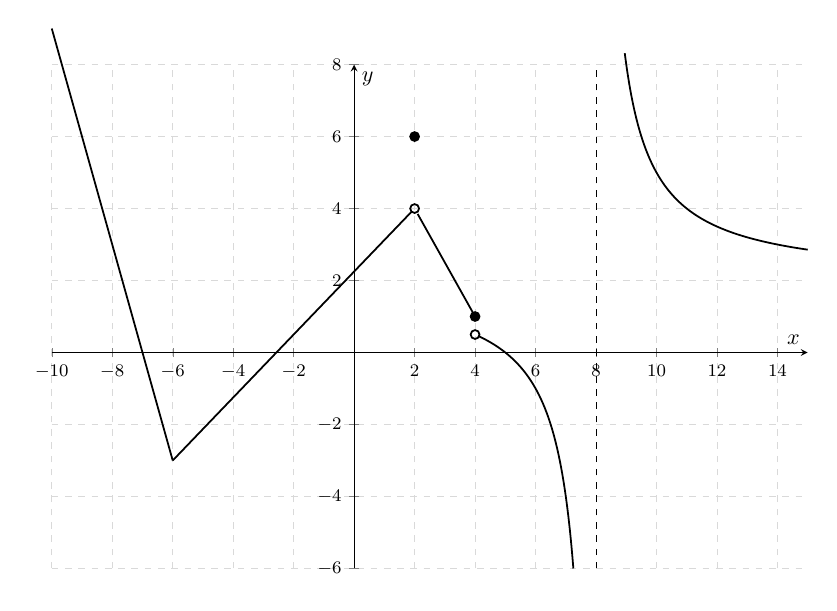
\begin{tikzpicture}[scale=0.8]
  \begin{axis}[
    width=12cm, height=8cm, scale only axis,
    axis x line=middle, axis y line=middle,
    xlabel={$x$},
    %xlabel style={at={(axis description cs:1,0)},anchor=west},
    ylabel={$y$},
    %ylabel style={at={(axis description cs:0,1)},anchor=south},
    xmin=-10, xmax=15, ymin=-6, ymax=8,
    xtick={-10,-8,...,14}, ytick={-6,-4,...,8},
    tick label style={font=\footnotesize},
    grid=both, grid style={dashed,gray!30},
    clip=false,
  ]
    % 1) curved branch f1(x) = (x+6)^2 - 4
    \addplot[thick,domain=-10:-6,samples=100] {-3*x -21};
    % 2) f2(x) = 7/8 x + 9/4
    \addplot[thick,domain=-6:1.9]
      {(7/8)*x + 9/4};
    % open peak at (2,4)
    \addplot[only marks,mark=o,thick] coordinates {(2,4)};
    % 3) f3(x) = -3/2 x + 7
    \addplot[thick,domain=2.1:4]
      {-1.5*x + 7};
    % closed end at (4,1)
    \addplot[only marks,mark=*,thick] coordinates {(4,1)};
    \addplot[only marks,mark=*,thick] coordinates {(2,6)};

    % vertical asymptote
    \draw[dashed] (axis cs:8,-6) -- (axis cs:8,8);
    % hyperbola f4(x)=2+6/(x-8) left of x=8
    \addplot[thick,domain=4.1:7.25,samples=200] {2 + 6/(x-8)};
    \addplot[only marks,mark=o,thick] coordinates {(4,0.5)};
    % hyperbola f4(x)=2+6/(x-8) right of x=8
    \addplot[thick,domain=8.95:15,samples=200] {2 + 6/(x-8)};
  \end{axis}
\end{tikzpicture}
\end{center}
\begin{tasks}
	\task
	Déterminer graphiquement
	\begin{multicols}{3}
		\begin{enumerate}	
		\item $\displaystyle{\lim_{x\rightarrow 2}f(x)}$ 
		\item $f(1)$
		\item $\displaystyle{\lim_{x\rightarrow -1}f(x)}$
		\item $\displaystyle{\lim_{x\rightarrow -\tfrac{13}{2}}f(x)}$
		\item $f(4)$
		\item $f(8)$
		\end{enumerate}
	\end{multicols}
	\task Représenter graphiquement une fonction $f$ satisfaisant toutes les conditions suivantes~:
	\begin{multicols}{3}	
	\begin{enumerate}
		\item $\displaystyle{\lim_{x\rightarrow -\infty}f(x)=3}$
		\item $\displaystyle{\lim_{x\rightarrow -2}f(x)=-\infty}$
		\item $\displaystyle{\lim_{x\rightarrow 0}f(x)=-2}$
		\item $f(-3)=2$
		\item $f(0)=4$
		\item $\displaystyle{\lim_{c\rightarrow +\infty}f(x)=2}$ 
		
	\end{enumerate}
	\end{multicols}
\end{tasks}
\end{activite}
\begin{activite}[label=acti:limdg]
	Limite à gauche et limite à droite
	\tcblower
	On considère à nouveau la représentation graphique de l'activité \ref{acti:limgraph}. Déterminer~:
	\begin{tasks}(4)
		\task $\displaystyle{\lim_{x\rightarrow 4^+}f(x)}$ 
		\task $\displaystyle{\lim_{x\rightarrow 4^-}f(x)}$ 
		\task $\displaystyle{\lim_{x\rightarrow 8^+}f(x)}$ 
		\task $\displaystyle{\lim_{x\rightarrow 8^-}f(x)}$ 
		\task $\displaystyle{\lim_{x\rightarrow 2^+}f(x)}$ 
		\task $\displaystyle{\lim_{x\rightarrow 2^-}f(x)}$ 
		\task $\displaystyle{\lim_{x\rightarrow 0^+}f(x)}$ 
		\task $\displaystyle{\lim_{x\rightarrow 0^-}f(x)}$ 
		
	\end{tasks}
\end{activite}


\begin{activite}[label=acti:type10]
	Limite infinie du type $«\,\dfrac{1}{0}\,»$
	\tcblower
Soit $f$ la fonction réelle définie par
\[
f(x)=\frac{x^2+x-6}{x^2-9}.
\]

\begin{tasks}(1)
\task Déterminer le domaine de définition de $f$.
\task Étudier ce qui se passe numériquement pour des valeurs de $x$ proches de $3$. Pour cela, calculer les images de $2{,}9$ ; $2,99$ ; $2,999$ ; $2,9999$ puis de $3,1$ ; $3,01$ ; $3,001$ et $3,0001$.
\begin{multicols}{2}
\begin{enumerate}
\item Que constate-t-on ?
\item Que peut-on dire de l’image de 3 ?
\item Quelle notation utiliser ?
\item Interpréter graphiquement.
\end{enumerate}
\end{multicols}
\task Esquisser une représentation graphique de $f$ (à l’aide de geogebra par exemple).
\task Calculer « directement », sans passer par des étapes intermédiaires, $\displaystyle\lim_{x\to 3}\frac{x^2+x-6}{x^2-9}$.
\task Calculer, si elles existent, les limites à gauche et à droite des fonctions suivantes lorsque $x$ tend vers $a$ et interpréter graphiquement les résultats :
\begin{multicols}{2}
\begin{enumerate}
\item $f(x)=\dfrac{3x-7}{x-2}$ et $a=2$
\item $f(x)=\dfrac{-3x+2}{x+2}$ et $a=-2$
\item $f(x)=\dfrac{3}{(x-1)^2}$ et $a=1$
\item $f(x)=\dfrac{5x}{(x+3)^3}$ et $a=-3$
\end{enumerate}
\end{multicols}
\end{tasks}
\end{activite}

\begin{activite}[label=acti:type00]
	Indétermination $«\,\dfrac{0}{0}\,»$
\tcblower
On considère à nouveau la fonction réelle $f$ définie par $f(x) = \dfrac{x^2 + x - 6}{x^2 - 9}$.

\begin{tasks}(1)
\task Étudier ce qui se passe numériquement pour des valeurs de $x$ proches de $-3$. Pour cela, calculer les images de $-3,1 ; -3,01 ; -3,001 ; -3,0001$ puis de $-2,9 ; -2,99 ; -2,999 ; -2,9999$.
\task Que constate-t-on ?
\task Que peut-on dire de l'image de $-3$ ?
\task Quelle notation utiliser ?
\task Interpréter graphiquement.
\end{tasks}

Reprendre la représentation graphique de $f$ obtenue à l'aide de GeoGebra. Cette représentation graphique précédente n'est pas totalement correcte... Pourquoi ?

Calculer « directement », sans passer par des étapes intermédiaires $\displaystyle\lim_{x \to -3} \dfrac{x^2 + x - 6}{x^2 - 9}$ et interpréter graphiquement.

Calculer si possible les limites suivantes et interpréter graphiquement :
\begin{tasks}(2)
\task $\displaystyle\lim_{x \to 0} \dfrac{5x^2 - 7x}{x}$
\task $\displaystyle\lim_{x \to -1} \dfrac{x^2 + x}{x + 1}$
\end{tasks}

Pourquoi parle-t-on d'indéterminations ?
\end{activite}

\begin{activite}[label=acti:limrac]
Indéterminations avec des racines
\tcblower
\begin{tasks}(2)
\task On considère la fonction $f$ définie par $f(x) = \dfrac{x - 3}{\sqrt{x} - \sqrt{3}}$. Calculer $\displaystyle\lim_{x \to 3} \dfrac{x - 3}{\sqrt{x} - \sqrt{3}}$ et interpréter graphiquement.
\task Calculer $\displaystyle\lim_{x \to 4} \dfrac{\sqrt{x} - 2}{x - 4}$ et interpréter graphiquement.
\end{tasks}
\end{activite}

\begin{activite}[label=acti:asyVert]{Asymptotes verticales}
\tcblower
\begin{tasks}(1)
  \task Définir et illustrer les notions d’asymptote verticale. 
  \task Vrai ou faux ? Justifier.
    \begin{enumerate}
      \item Une fonction peut avoir plusieurs asymptotes verticales ?
      \item La courbe représentative d’une fonction ne coupe jamais son asymptote verticale.
    \end{enumerate}
  \task Déterminer toutes les asymptotes verticales de la fonction \(f\) déterminée par
  \[
    f(x)=\dfrac{x^2 - x}{2x^2 + 2x - 4}
  \]
  et interpréter graphiquement.
\end{tasks}
\end{activite}

\begin{activite}[label=acti:liminf]
	Limites à l'infini
	\tcblower
	\begin{tasks}
	\task On considère la fonction $f$ définie par $f(x)=x^2+x-6$.
\begin{multicols}{3}
		\begin{enumerate}
\item Quel sens donner à $\displaystyle\lim_{x\to +\infty}f(x)\,$ ?
\item Comment calculer $\displaystyle\lim_{x\to +\infty}f(x)\,$ ?
\item Et $\displaystyle\lim_{x\to -\infty}f(x)\,$ ?
		\end{enumerate}
	\end{multicols}
	\task Énoncer et discuter ce qu'on entend par «~limites à l'infini~».
	\task Calculer (si possible) les limites à l'infini suivantes en utilisant l'aglèbre de l'infini. 

\begin{multicols}{3}
\begin{enumerate}
\item $\displaystyle\lim_{x\to +\infty}\bigl(x^3+5x+3\bigr)$
\item $\displaystyle\lim_{x\to -\infty}\bigl(x^3+5x+10^{100}\bigr)$
\item $\displaystyle\lim_{x\to +\infty}\frac{2}{3x^2-4}$
\end{enumerate}
\end{multicols}
	\end{tasks}
\end{activite}

\begin{activite}[label=acti:indInf]
Indéterminations avec l'infini
\tcblower
On considère la fonction $f$ définie par $f(x) = \dfrac{x^2 + x - 6}{x^2 - 9}$.

Calculer $\displaystyle\lim_{x \to +\infty} \dfrac{x^2 + x - 6}{x^2 - 9}$ et $\displaystyle\lim_{x \to -\infty} \dfrac{x^2 + x - 6}{x^2 - 9}$ et interpréter graphiquement.

Calculer si possible les limites suivantes et interpréter graphiquement :

\begin{tasks}(3)
\task $\displaystyle\lim_{x \to +\infty} \dfrac{2x^2 - 9x}{3x^2 - 5x - 4}$
\task $\displaystyle\lim_{x \to +\infty} \dfrac{3x^2 - x + 1}{x + 3}$
\task $\displaystyle\lim_{x \to +\infty} \dfrac{2x^2 - x}{5x + 2}$
\task $\displaystyle\lim_{x \to +\infty} (x^2 + x)$
\task $\displaystyle\lim_{x \to +\infty} (2x - x^2)$
\end{tasks}
\end{activite}

\begin{activite}[label=acti:asyhor]{Asymptotes horizontales}
\tcblower
\begin{tasks}(1)
  \task Définir et illustrer les notions d’asymptote horizontale.
  \task Vrai ou faux ? Justifier.
    \begin{enumerate}
      \item Une fonction peut avoir plusieurs asymptotes horizontales ?
      \item La courbe représentative d’une fonction ne coupe jamais son asymptote horizontale.
    \end{enumerate}
  \task Déterminer les asymptotes horizontales de la fonction \(f\) déterminée par
  \[
    f(x)=\dfrac{x^2 - x}{2x^2 + 2x - 4}
  \]
  et interpréter graphiquement.
\end{tasks}
\end{activite}



\begin{activite}[label=acti:asyconcl]{Tout en un}
\tcblower
\begin{tasks}(1)
  \task Déterminer toutes les asymptotes de la fonction \(f\) définie par
  \[
    f(x)=\dfrac{2x^3+4x^2-2x}{-x^3+x^2+x-1}
  \]
  et interpréter graphiquement.
\end{tasks}
\end{activite}

\begin{activite}[label=acti:asydouble]{Double asymptote}
\tcblower
\begin{tasks}(1)
  \task Déterminer toutes les asymptotes de la fonction \(f\) définie par
  \[
    f(x)=x-\sqrt{x^2-1}
  \]
  et interpréter graphiquement.
\end{tasks}
\end{activite}

\begin{activite}[label=acti:constrgraph]
Graphiquement
\tcblower
Représenter graphiquement une (unique) fonction $f$ de votre choix qui vérifie simultanément toutes les conditions suivantes :

\begin{tasks}(2)
\task L'ensemble $D_f$ des zéros de $f$ est $\{-2;4\}$
\task L'image de $0$ est $-2$
\task $\displaystyle\lim_{x \to 1} f(x) = -\infty$
\task $\displaystyle\lim_{x \to +\infty} f(x) = +\infty$
\task $\displaystyle\lim_{x \to +\infty} f(x) = 4$
\task $\displaystyle\lim_{x \to +\infty} f(x) = 2$ et $f(-4) = -2$
\end{tasks}
\end{activite}

\begin{activite}{Une limite trigonométrique importante}
\tcblower
\begin{tasks}(1)
\task On considère la fonction $f$ déterminée par $f(x) = \dfrac{\sin(x)}{x}$
\begin{enumerate}
\item Déterminer $D_f$ et $Z_f$.
\item D'après votre intuition, et/ou à l'aide de la calculatrice:
\item Que pensez-vous de $\displaystyle\lim_{x \to 0} f(x)$ et de ? $\displaystyle\lim_{x \to 0} f(x)$
\item Existe-t-il une asymptote horizontale pour cette fonction?
\item Pouvez-vous justifier ces réponses?
\end{enumerate}

\task On s'intéresse maintenant à $\displaystyle\lim_{x \to 0} f(x)$
\begin{enumerate}
\item Conjecturer une valeur pour cette limite, à partir d'essais numériques avec la calculatrice.
\item Proposer une représentation graphique de $f$ sur la base des informations recueillies jusqu'à présent.
\end{enumerate}

\task Que penser de $\displaystyle\lim_{y \to 0} \dfrac{\sin(y^2)}{y^2}$, de $\displaystyle\lim_{z \to 0} \dfrac{\sin(z)}{-z}$, de $\displaystyle\lim_{x-a \to 0} \dfrac{\sin(x-a)}{x-a}$, de $\displaystyle\lim_{x \to a} \dfrac{\sin(x-a)}{x-a}$ ?

\task Calculer $\displaystyle\lim_{x \to 0} \dfrac{\cos(x)}{x}$ et $\displaystyle\lim_{x \to 0} \dfrac{\tan(x)}{x}$
\end{tasks}
\end{activite}
\begin{activite}{Indéterminations trigonométriques de type « $\dfrac{0}{0}$ »}
\tcblower
\begin{tasks}(1)
\task Calculer :
\begin{multicols}{3}
\begin{enumerate}
\item $\displaystyle\lim_{x \to 0} \dfrac{\sin(12x)}{6x}$
\item $\displaystyle\lim_{x \to 0} \dfrac{\sin(8x)}{10x^2}$
\item $\displaystyle\lim_{x \to 2} \dfrac{\sin(x-2)}{3x-6}$
\item $\displaystyle\lim_{x \to 0} \dfrac{\tan(12x)}{6x}$
\item $\displaystyle\lim_{x \to 2} \dfrac{6-3x}{\sin(x-2)}$
\item $\displaystyle\lim_{x \to 2} \dfrac{\cos(x-2)}{3x-6}$
\end{enumerate}
\end{multicols}
\end{tasks}
\end{activite}

\newpage

\section{Exercices}
Dans les corrigés vous trouverez seulement des éléments de réponses. {\bfseries Une réponse détaillée et justifiée} à l'aide des résultats du cours est attendue. L'enseignant est là pour valider votre réponse et vérifier votre rédaction. {\bfseries En évaluation, une réponse qui n'est pas justifiée selon les attentes ne recueillera pas de point.} 

\subsection{Continuité}
\insertexo{1n93r}{false}{both}
\insertexo{59swy}{false}{both}
\insertexo{qp2mw}{false}{both}
\insertexo{6csvs}{false}{both}
\subsection{Limites en un nombre}
\insertexo{4dptb}{false}{both}
\insertexo[exo:p1f]{g4gbb}{false}{both}
\insertexo{n9sxp}{false}{both}
\insertexo[exo:p2d]{tecfn}{false}{both}
\insertexo{wnd21}{false}{both}
\insertexo{3vr28}{false}{both}
\insertexo{c3uc9}{false}{both}
\insertexo{1bqh9}{false}{both}
\insertexo{myjcq}{false}{both}
\insertexo{dpjwk}{false}{both}
\insertexo{97ryj}{false}{both}
\insertexo{n1axs}{false}{both}

\insertexo{gb3ag}{false}{both}
\insertexo{5911p}{false}{both}

\insertexo{hsytn}{false}{both}
\subsubsection{Limites infinies « $\dfrac{1}{0}$ » et indétermination du type « $\dfrac{0}{0}$ »}

\insertexo[exo:p1d]{vyj67}{false}{both}
\insertexo{ac9v2}{false}{both}
\insertexo{98752}{false}{both}
\insertexo{gg7hk}{false}{both}
\insertexo{f7dft}{false}{both}
\insertexo{u44h9}{false}{both}
\insertexo{pp62m}{false}{both}
\insertexo{b3p6g}{false}{both}
\insertexo{n41yn}{false}{both}
\insertexo{8j18h}{false}{both}
\insertexo{yhzh8}{false}{both}
\insertexo{9yqnb}{false}{both}
%--> corrigés vérifiés après ici.
\insertexo{k3bry}{false}{both}
\insertexo{1w6s3}{false}{both}
\insertexo{nxc2s}{false}{both}
\subsubsection{Asymptotes verticales}
\insertexo{89av7}{false}{both}
\insertexo{1w3pd}{false}{both}
\subsection{Limites en l'infini}
\insertexo{x5h3r}{false}{exo}
\insertexo{n9qmn}{false}{exo}
\insertexo{t4gwt}{false}{exo}
\insertexo{bqknk}{false}{exo}
\insertexo{du7be}{false}{exo}
\insertexo{6qym1}{false}{exo}
\insertexo{aatq8}{false}{exo}
\insertexo{gm9uk}{false}{exo}
\insertexo{taje8}{false}{exo}
\insertexo{y4dv7}{false}{exo}
\insertexo{y4385}{false}{exo}
\insertexo{2at6d}{false}{exo}
%MA2\insertexo{us8px}{false}{exo}
\insertexo{5en1r}{false}{exo}
\insertexo{zu8c5}{false}{exo}
\insertexo{1gayt}{false}{exo}
%MA2\insertexo{pe1ew}{false}{exo}
%MA2\insertexo{mj5qq}{false}{exo}
%MA2\insertexo{hgcu8}{false}{exo}
%MA2\insertexo{ek51g}{false}{exo}
%MA2\insertexo{955md}{false}{exo}
%MA2\insertexo{mkn1h}{false}{exo}
%MA2\insertexo{pzy7s}{false}{exo}
\insertexo{3yjzh}{false}{exo}

\subsection{Limites de fonctions trigonométriques}
\insertexo{byf5j}{false}{exo}
\insertexo{h9w1s}{false}{exo}
\insertexo{jqhm4}{false}{exo}


%Pas inclus 
%\insertexo[exo:p1d]{vyj67}{false}{exo}
%\insertexo{4dptb}{false}{exo}
%\insertexo[exo:p1f]{g4gbb}{false}{exo}
%%\insertexo{extez}{false}{exo}
%%\insertexo{znghn}{false}{exo}
%\insertexo[exo:p2d]{tecfn}{false}{exo}
%%\insertexo{fazjq}{false}{exo}
%\insertexo{f7dft}{false}{exo}
%\insertexo{ac9v2}{false}{exo}
%\insertexo{nxc2s}{false}{exo}
%\insertexo{n9qmn}{false}{exo}
%\insertexo{bqknk}{false}{exo}
%\insertexo{gg7hk}{false}{exo}
%\insertexo{n41yn}{false}{exo}
%\insertexo{8j18h}{false}{exo}
%\insertexo{1w3pd}{false}{exo}
%\insertexo{x5h3r}{false}{exo}
%\insertexo{1bqh9}{false}{exo}
%\insertexo{du7be}{false}{exo}
%\insertexo{k3bry}{false}{exo}
%\insertexo{gm9uk}{false}{exo}
%\insertexo{taje8}{false}{exo}
%\insertexo{3vr28}{false}{exo}
%\insertexo{gb3ag}{false}{exo}
%\insertexo{c3uc9}{false}{exo}
%\insertexo{myjcq}{false}{exo}
%\insertexo{dpjwk}{false}{exo}
%\insertexo{97ryj}{false}{exo}
%\insertexo{n1axs}{false}{exo}
%\insertexo{wnd21}{false}{exo}
%\insertexo{98752}{false}{exo}
%\insertexo{t4gwt}{false}{exo}
%\insertexo{1w6s3}{false}{exo}
%\insertexo{yhzh8}{false}{exo}
%\insertexo{9yqnb}{false}{exo}
%\insertexo{byf5j}{false}{exo}
%\insertexo{h9w1s}{false}{exo}
%\insertexo{jqhm4}{false}{exo}
%\insertexo{1n93r}{false}{exo}
%\insertexo{qp2mw}{false}{exo}
%\insertexo{6qym1}{false}{exo}
%\insertexo{aatq8}{false}{exo}
\newpage
\section{Pistes pour réviser}
\begin{itemize}
	\item Quelles sont les trois conditions qu'une fonction doit satisfaire {\bfseries simultanément} pour être continue en un point~? Donner des exemples de fonctions qui satisfont seulement deux des trois conditions.
	\item Quelle est la première étape à effectuer dans tout calcul de limite~?
	\item Une limite peut être déterminée ou indéterminée, en un nombre ou en l'infini. Donner des exemples de chacun de ces cas. 
	\item Qu'est-ce qu'une indétermination~? Quels sont les différents cas, leurs particularités et les différentes manières de les lever~? Donner des exemples.
	\item Quelle technique a-t-on à diposition pour calculer une limite qui contient une expression littérale avec une racine~?
%MA2	\item Quelles sont les différences entre les asymptotes verticales, horizontales et obliques~? Expliquer et donner des exemples.
	\item Donner des conditions pour l'existence d'asymptotes verticales. Exemples. 
	\item Donner des conditions pour l'existence d'asymptotes horizontales. Exemples.
%MA2	\item Donner des conditions pour l'existence d'asymptotes obliques. Exemples.
	\item Quelles sont les deux façons qui ont étudiées pour calculer une limite trigonométrique~? Exemples. 
\end{itemize}
 \nocite{*}
 \vspace{-10pt}
\defbibnote{myprenote}{Les sources suivantes ont majoritairement été utilisées pour construire ce cours. Les exercices et activités proviennent également principalement de ces ouvrages. D'autres exercices ont été adaptés ou sont inspirés de ressources partagées par des collègues ou trouvées sur internet. Leur contribution mineure les exclut de cette liste.}
 \printbibliography[prenote=myprenote,title={Sources du cours}] 
\end{document}

